\documentclass[xcolor=dvipsnames]{beamer} 
\usepackage[utf8]{inputenc}
\usepackage[T1]{fontenc}
\usepackage{lmodern}
\usepackage[ngerman]{babel}
\usepackage{textcomp}
\usepackage{graphicx}
\usepackage{caption3}
\usetheme{CambridgeUS}
\usecolortheme{whale}
\setbeamercolor{frametitle}{fg=subsection in head/foot.bg}
\setbeamercovered{transparent}
\usepackage{epstopdf}
\usepackage{pifont}% http://ctan.org/pkg/pifont
\newcommand{\cmark}{\ding{51}}%Häkchen
\newcommand{\xmark}{\ding{55}}%Kreuz
\usepackage{amssymb}
\usepackage{xcolor}

%Die Maße einer Folie in der Beamer-Präsentation betragen 128x96mm%

\title{Diplomarbeit}
\subtitle{Zusammenhang zwischen Makrophytobenthos und Sedimentstruktur in flachen Küstengewässern der deutschen Ostsee}
\author{Antje Kerkow}
\institute[Universität Greifswald]{Studiengang Landschaftsökologie und Naturschutz}
\date{13.5.2014}
\AtBeginSubsection

\begin{document}

\begin{frame}
\titlepage
\end{frame}

\section{Einleitung}
\begin{frame}
\frametitle{Definitionen}
\begin{columns}
\begin{column}{5.5cm}
\begin{figure}
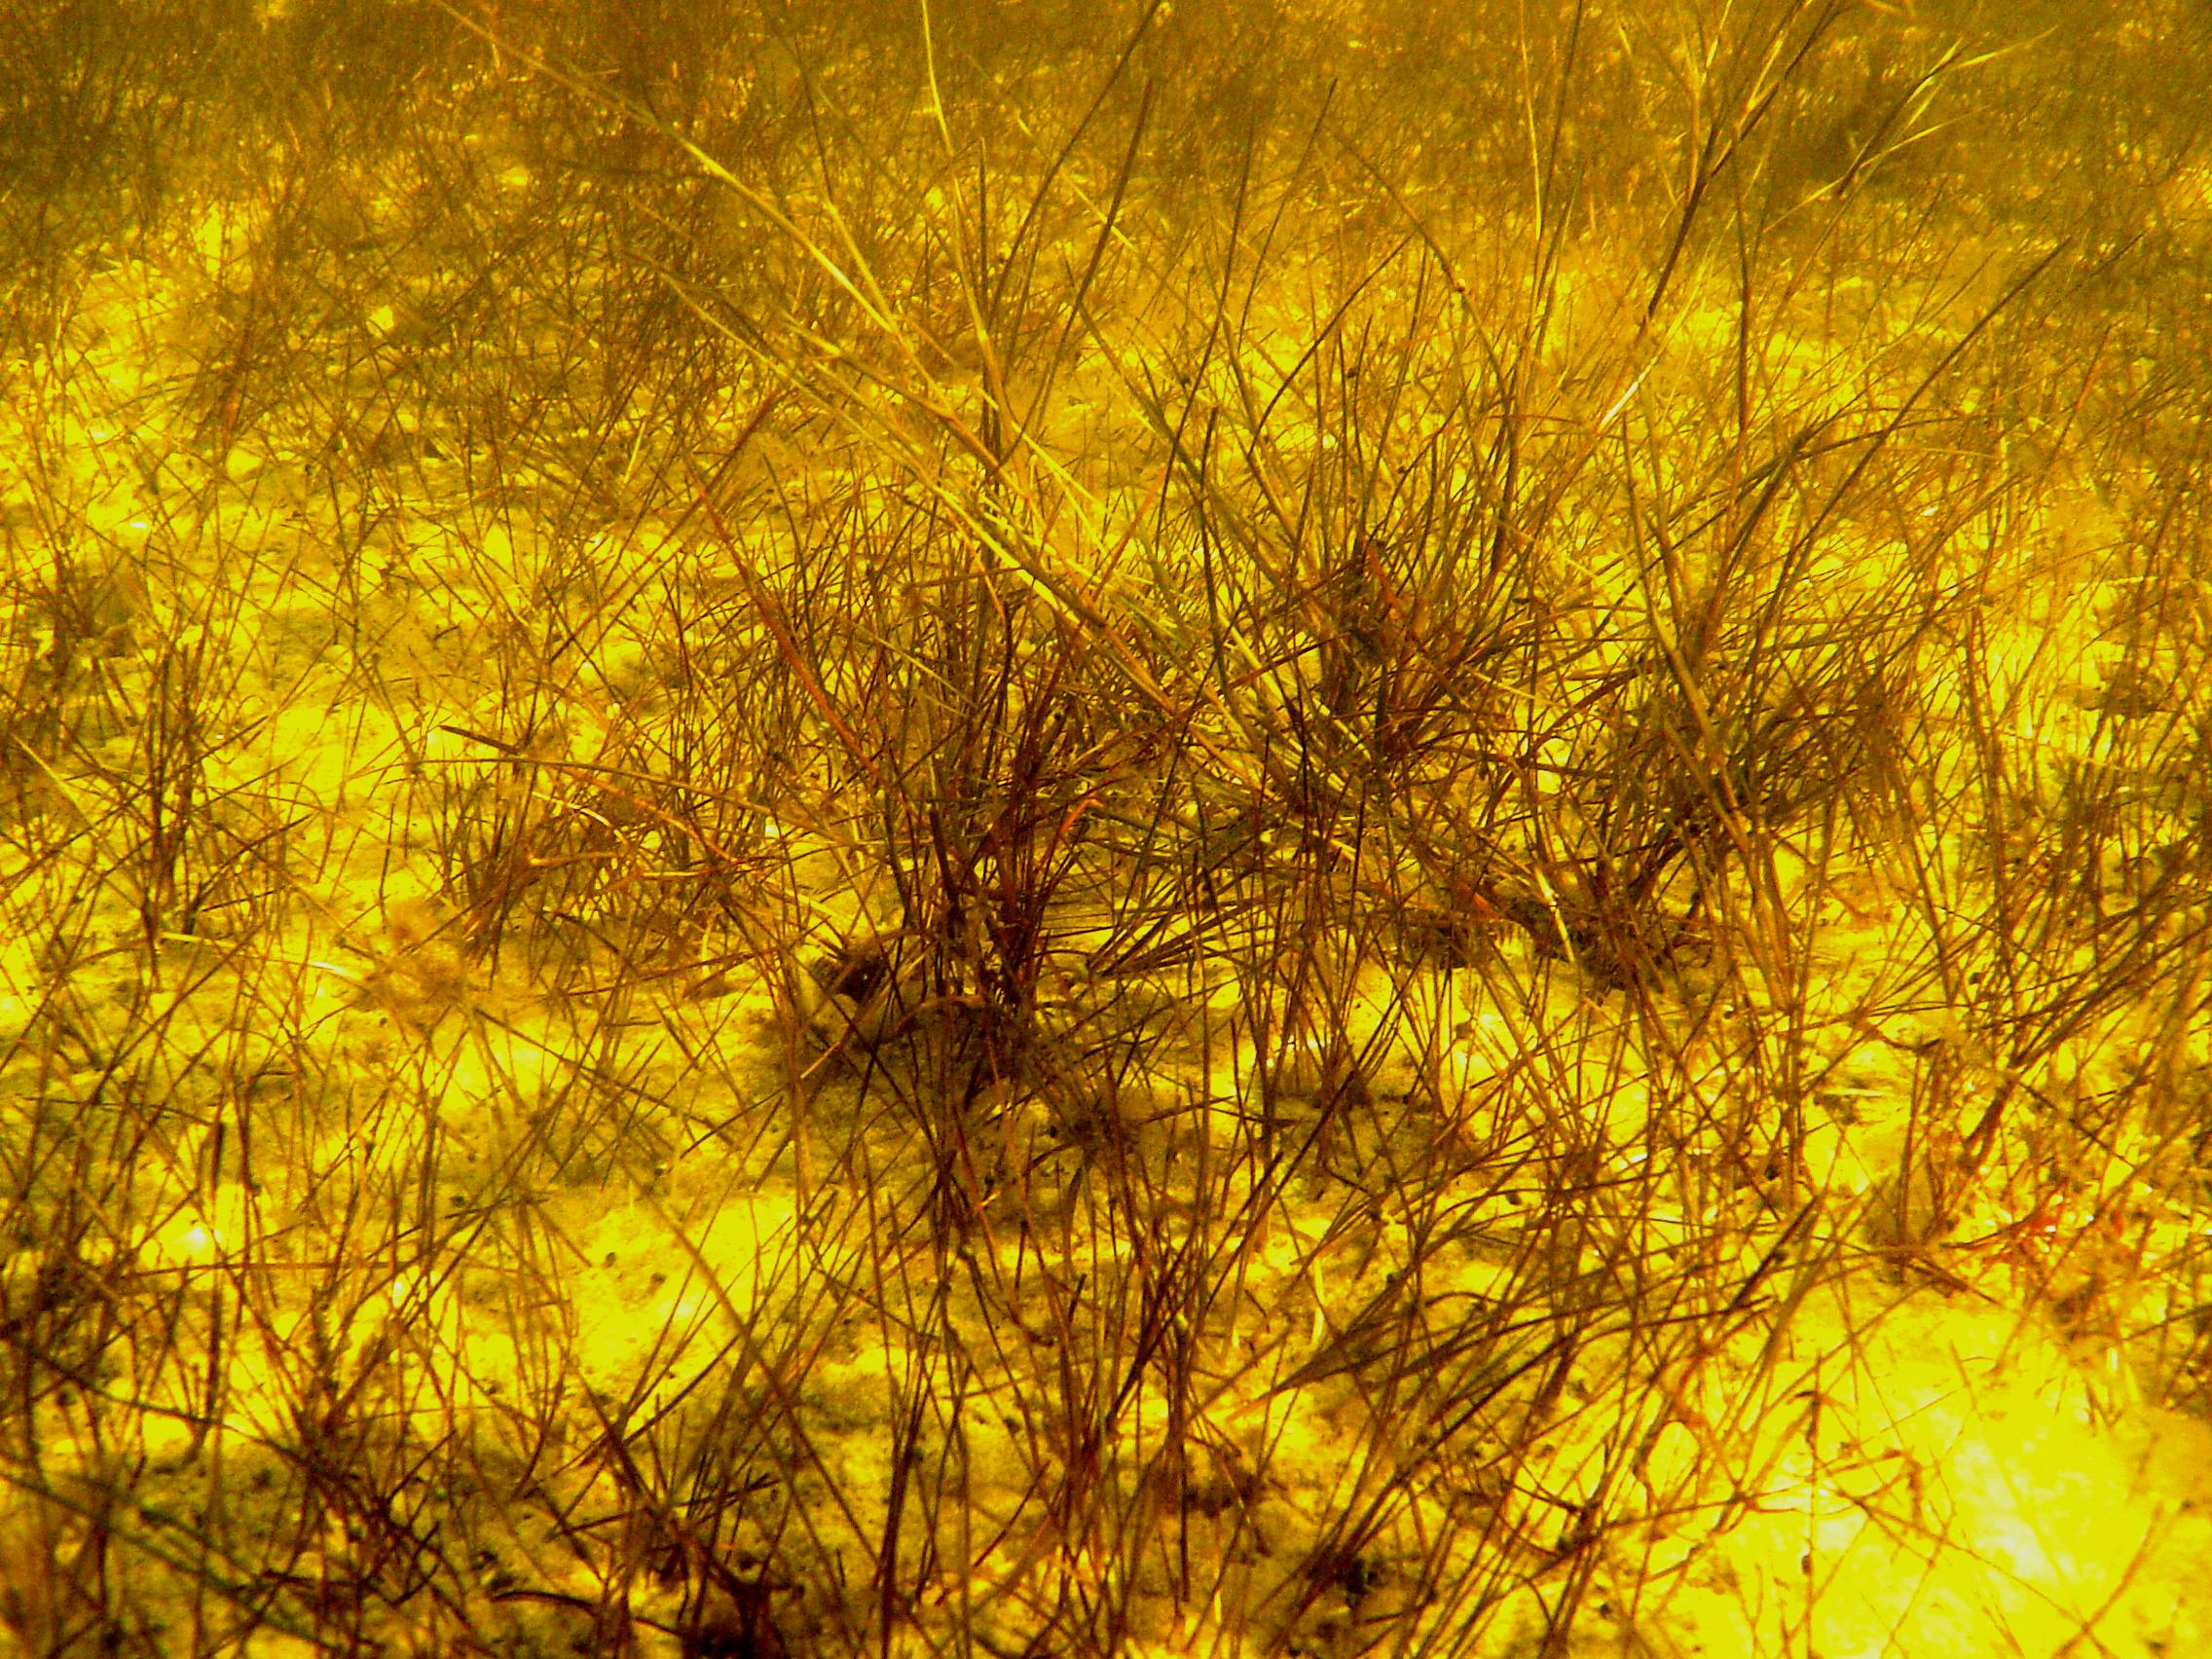
\includegraphics[height=40mm]{images/Fotos/makrophytobenthos.jpg}

Makrophytobenthos
\end{figure}
\end{column}
\begin{column}{5.5cm}
\begin{figure}
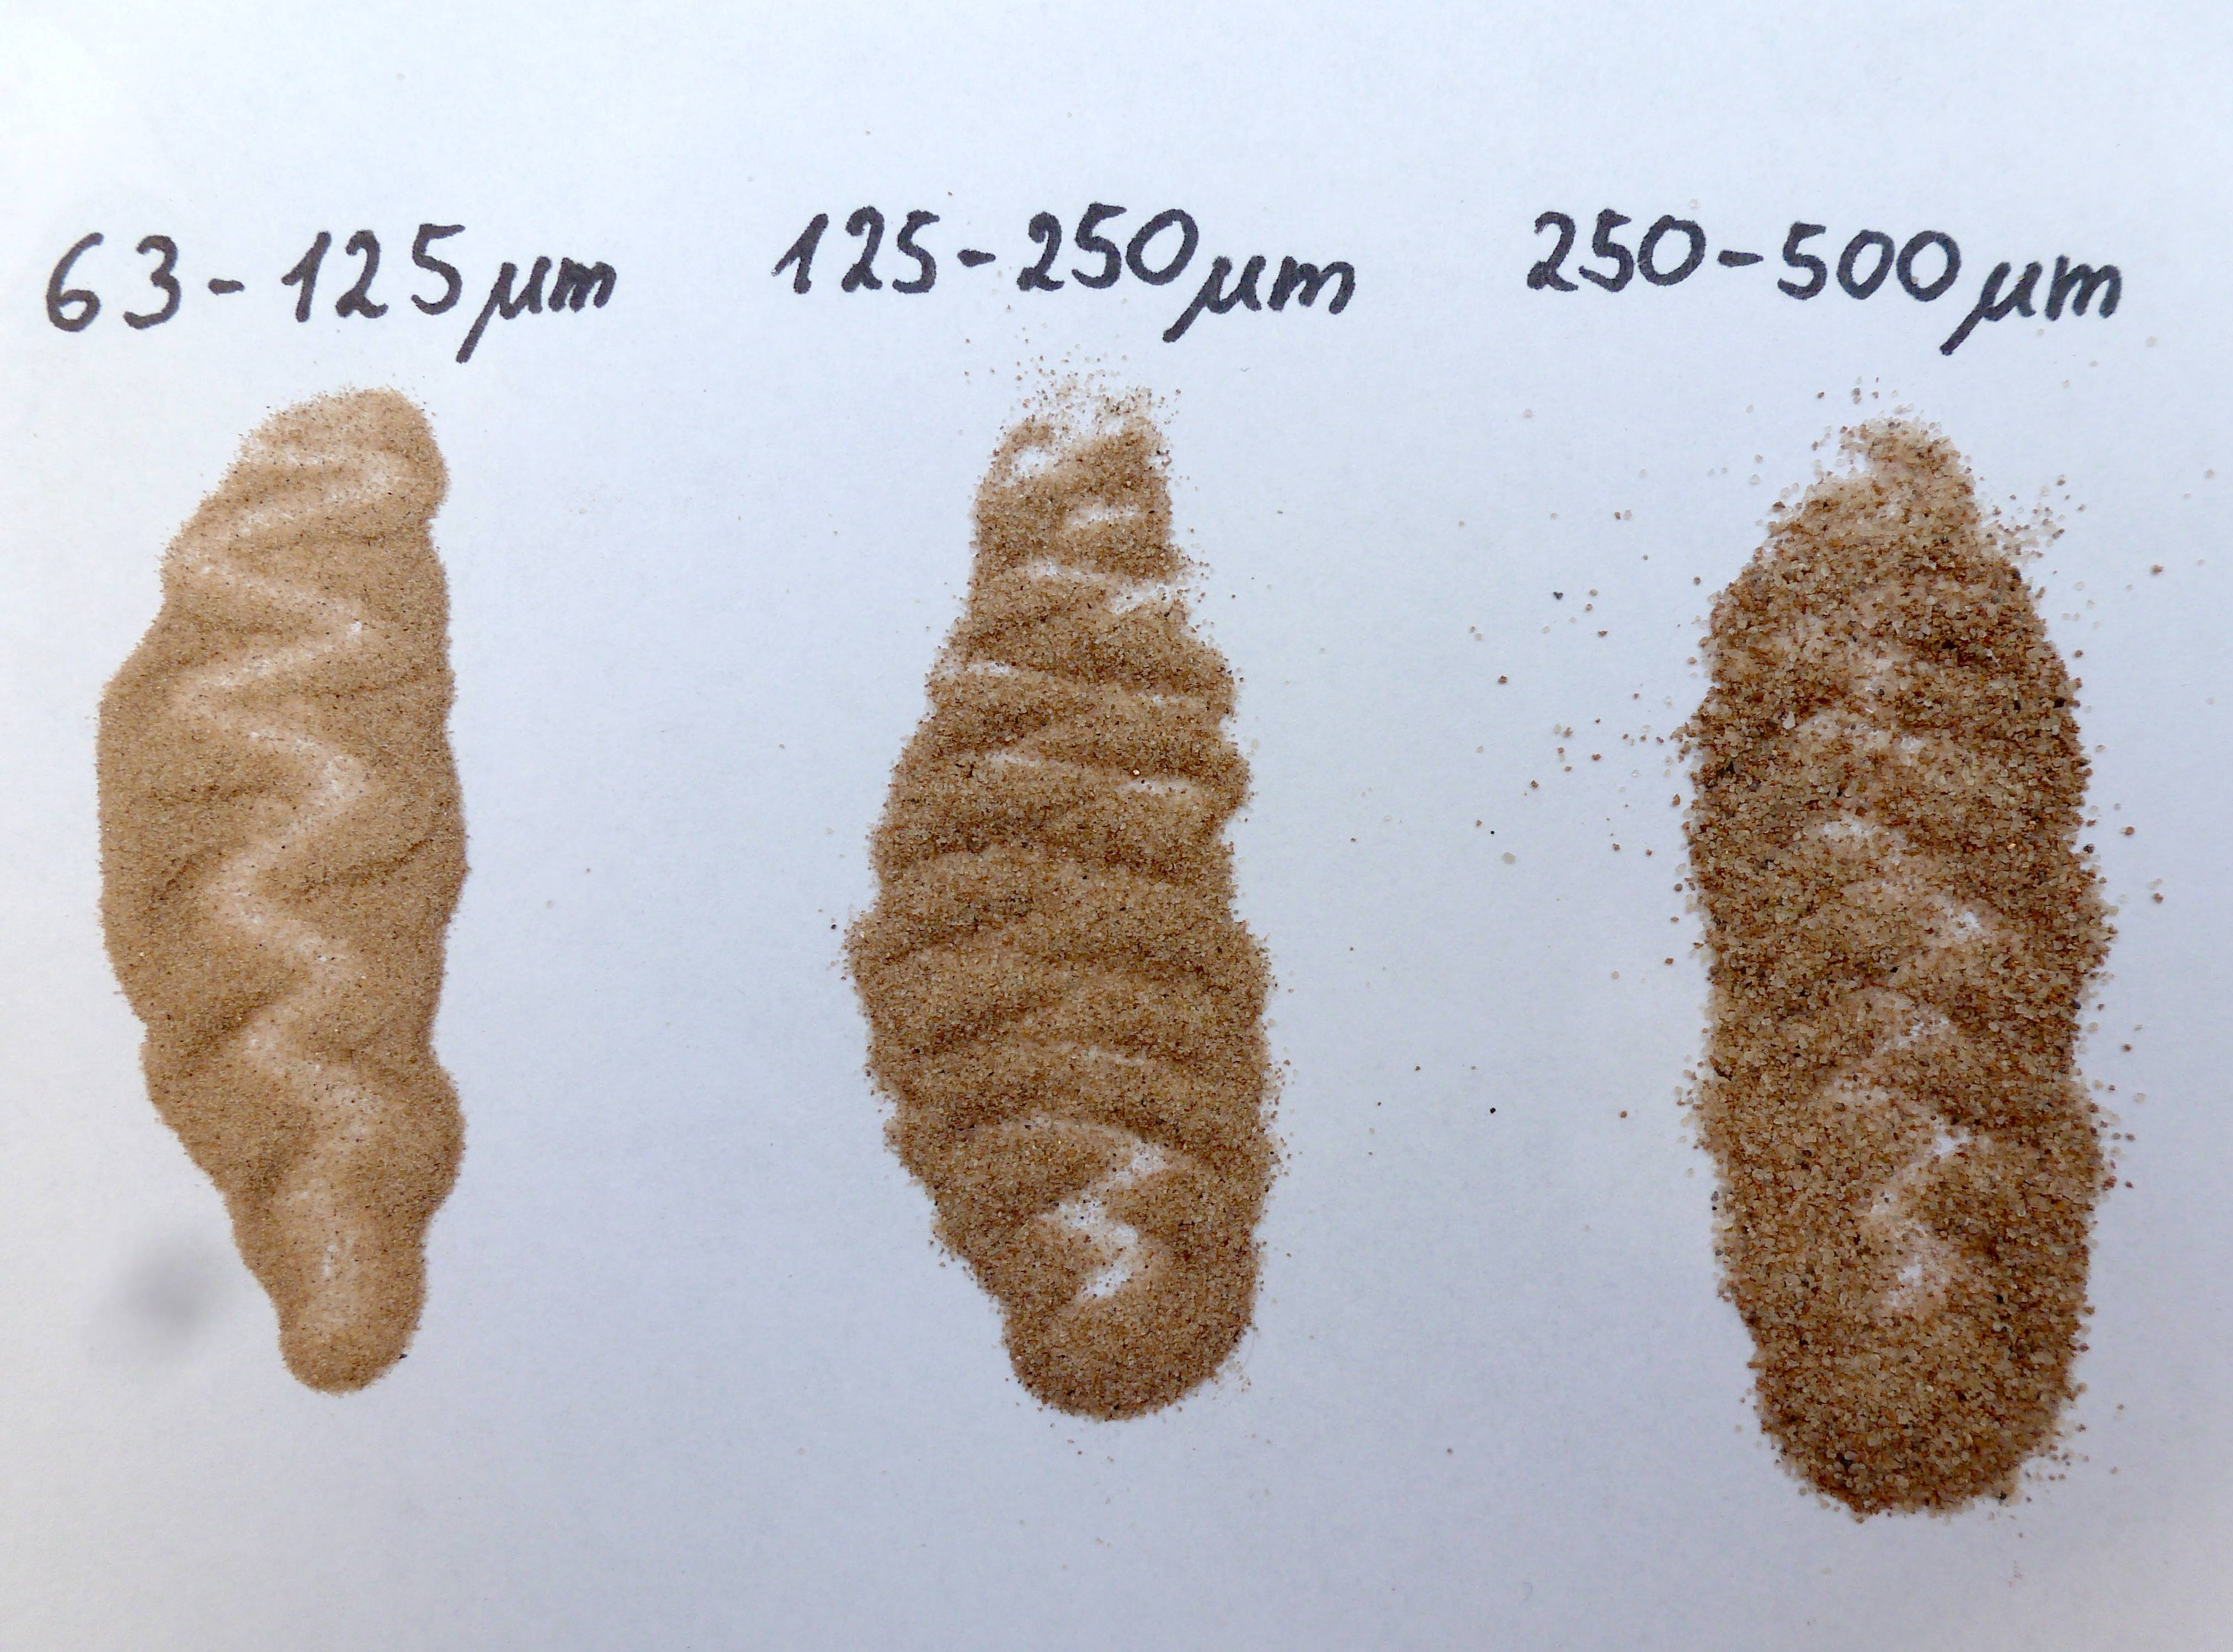
\includegraphics[height=40mm]{images/Fotos/korngroessen.jpg}

Sedimentstruktur
\end{figure}
\end{column}
\end{columns}
\end{frame}

\begin{frame}
\begin{figure}
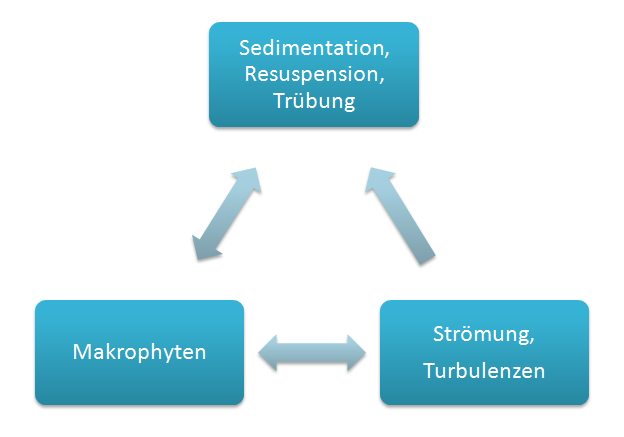
\includegraphics[width=0.7\textwidth]{images/Schema_Pfl_Sedim_Strm}
\end{figure}
\end{frame}

\begin{frame}
\frametitle{Fragestellungen dieser Arbeit}
\begin{enumerate}
\item Ist in dichten Makrophytenbeständen das Sediment feiner als auf freien/ spärlich besiedelten Flächen?
\pause
\item Ist der organische Gehalt der Sedimente in den dichten Beständen höher?
\pause
\item Verändert sich die Vegetationsstruktur im Jahresverlauf?
\pause
\item Verändert sich die mittlere Korngröße, der Feinpartikelanteil und der organische Gehalt der Sedimente im Jahresverlauf? 
\end{enumerate}
\end{frame}

\section{Untersuchungsgebiete}
\subsection{Alle Stationen entlang des Salzgradienten}
%\begin{frame}
%\frametitle{Alle Stationen entlang des Salzgradienten}
%\begin{figure}
%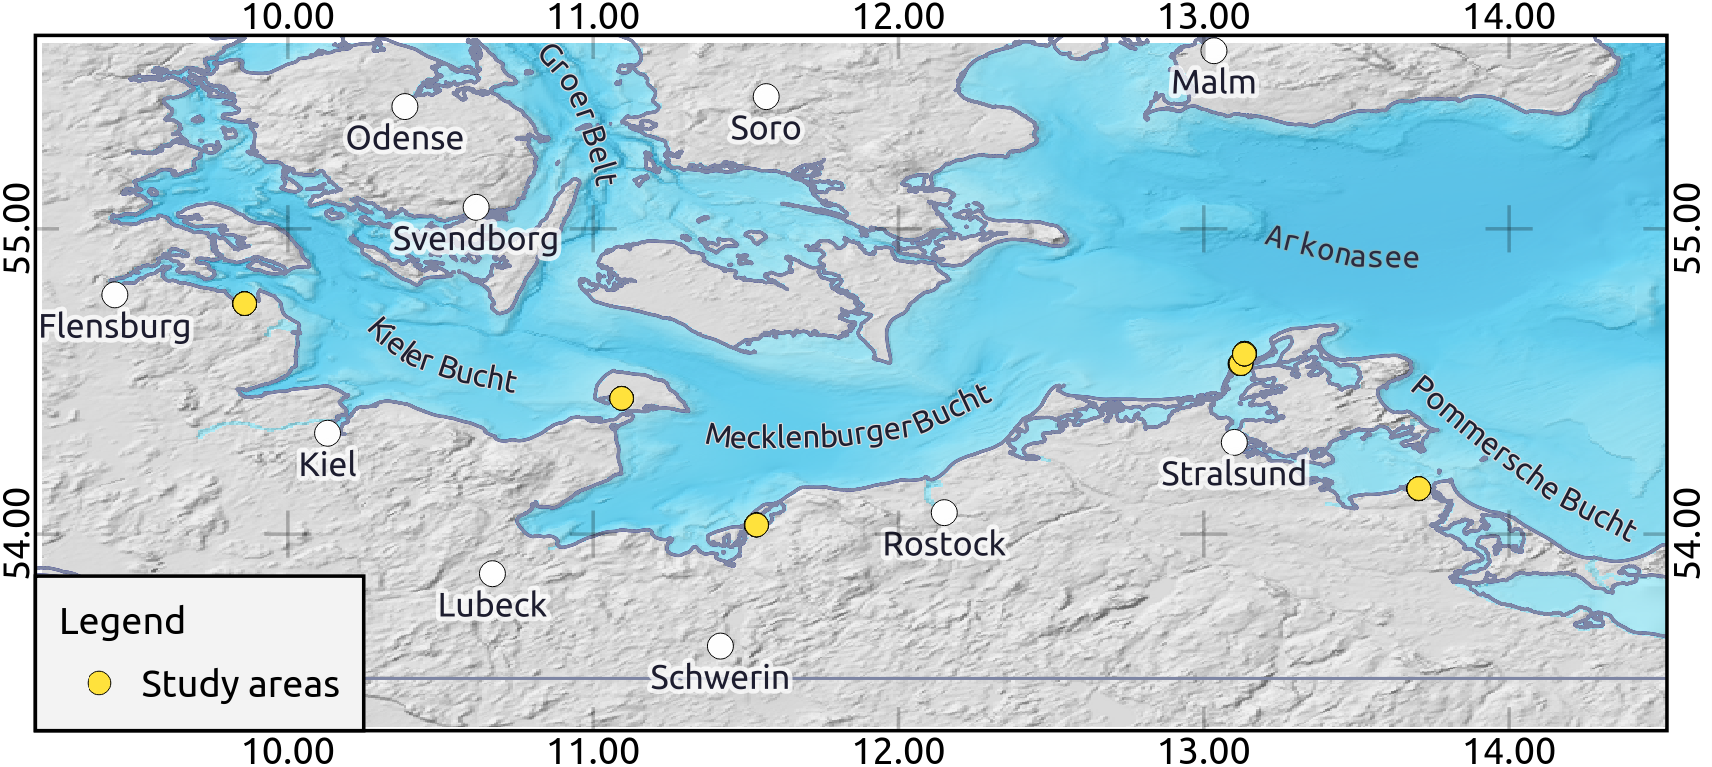
\includegraphics[scale=0.24]{images/Uebersicht.png}
%\end{figure}
%\begin{center}
%Geltinger B., Orther B., Salzhaff, Hiddenseer B., Spandowerh.Wiek
%\end{center}
%\end{frame}

\subsection{Hiddenseer Standorte}

\begin{frame}
\frametitle{Untersuchungsgebiet}
\begin{figure}
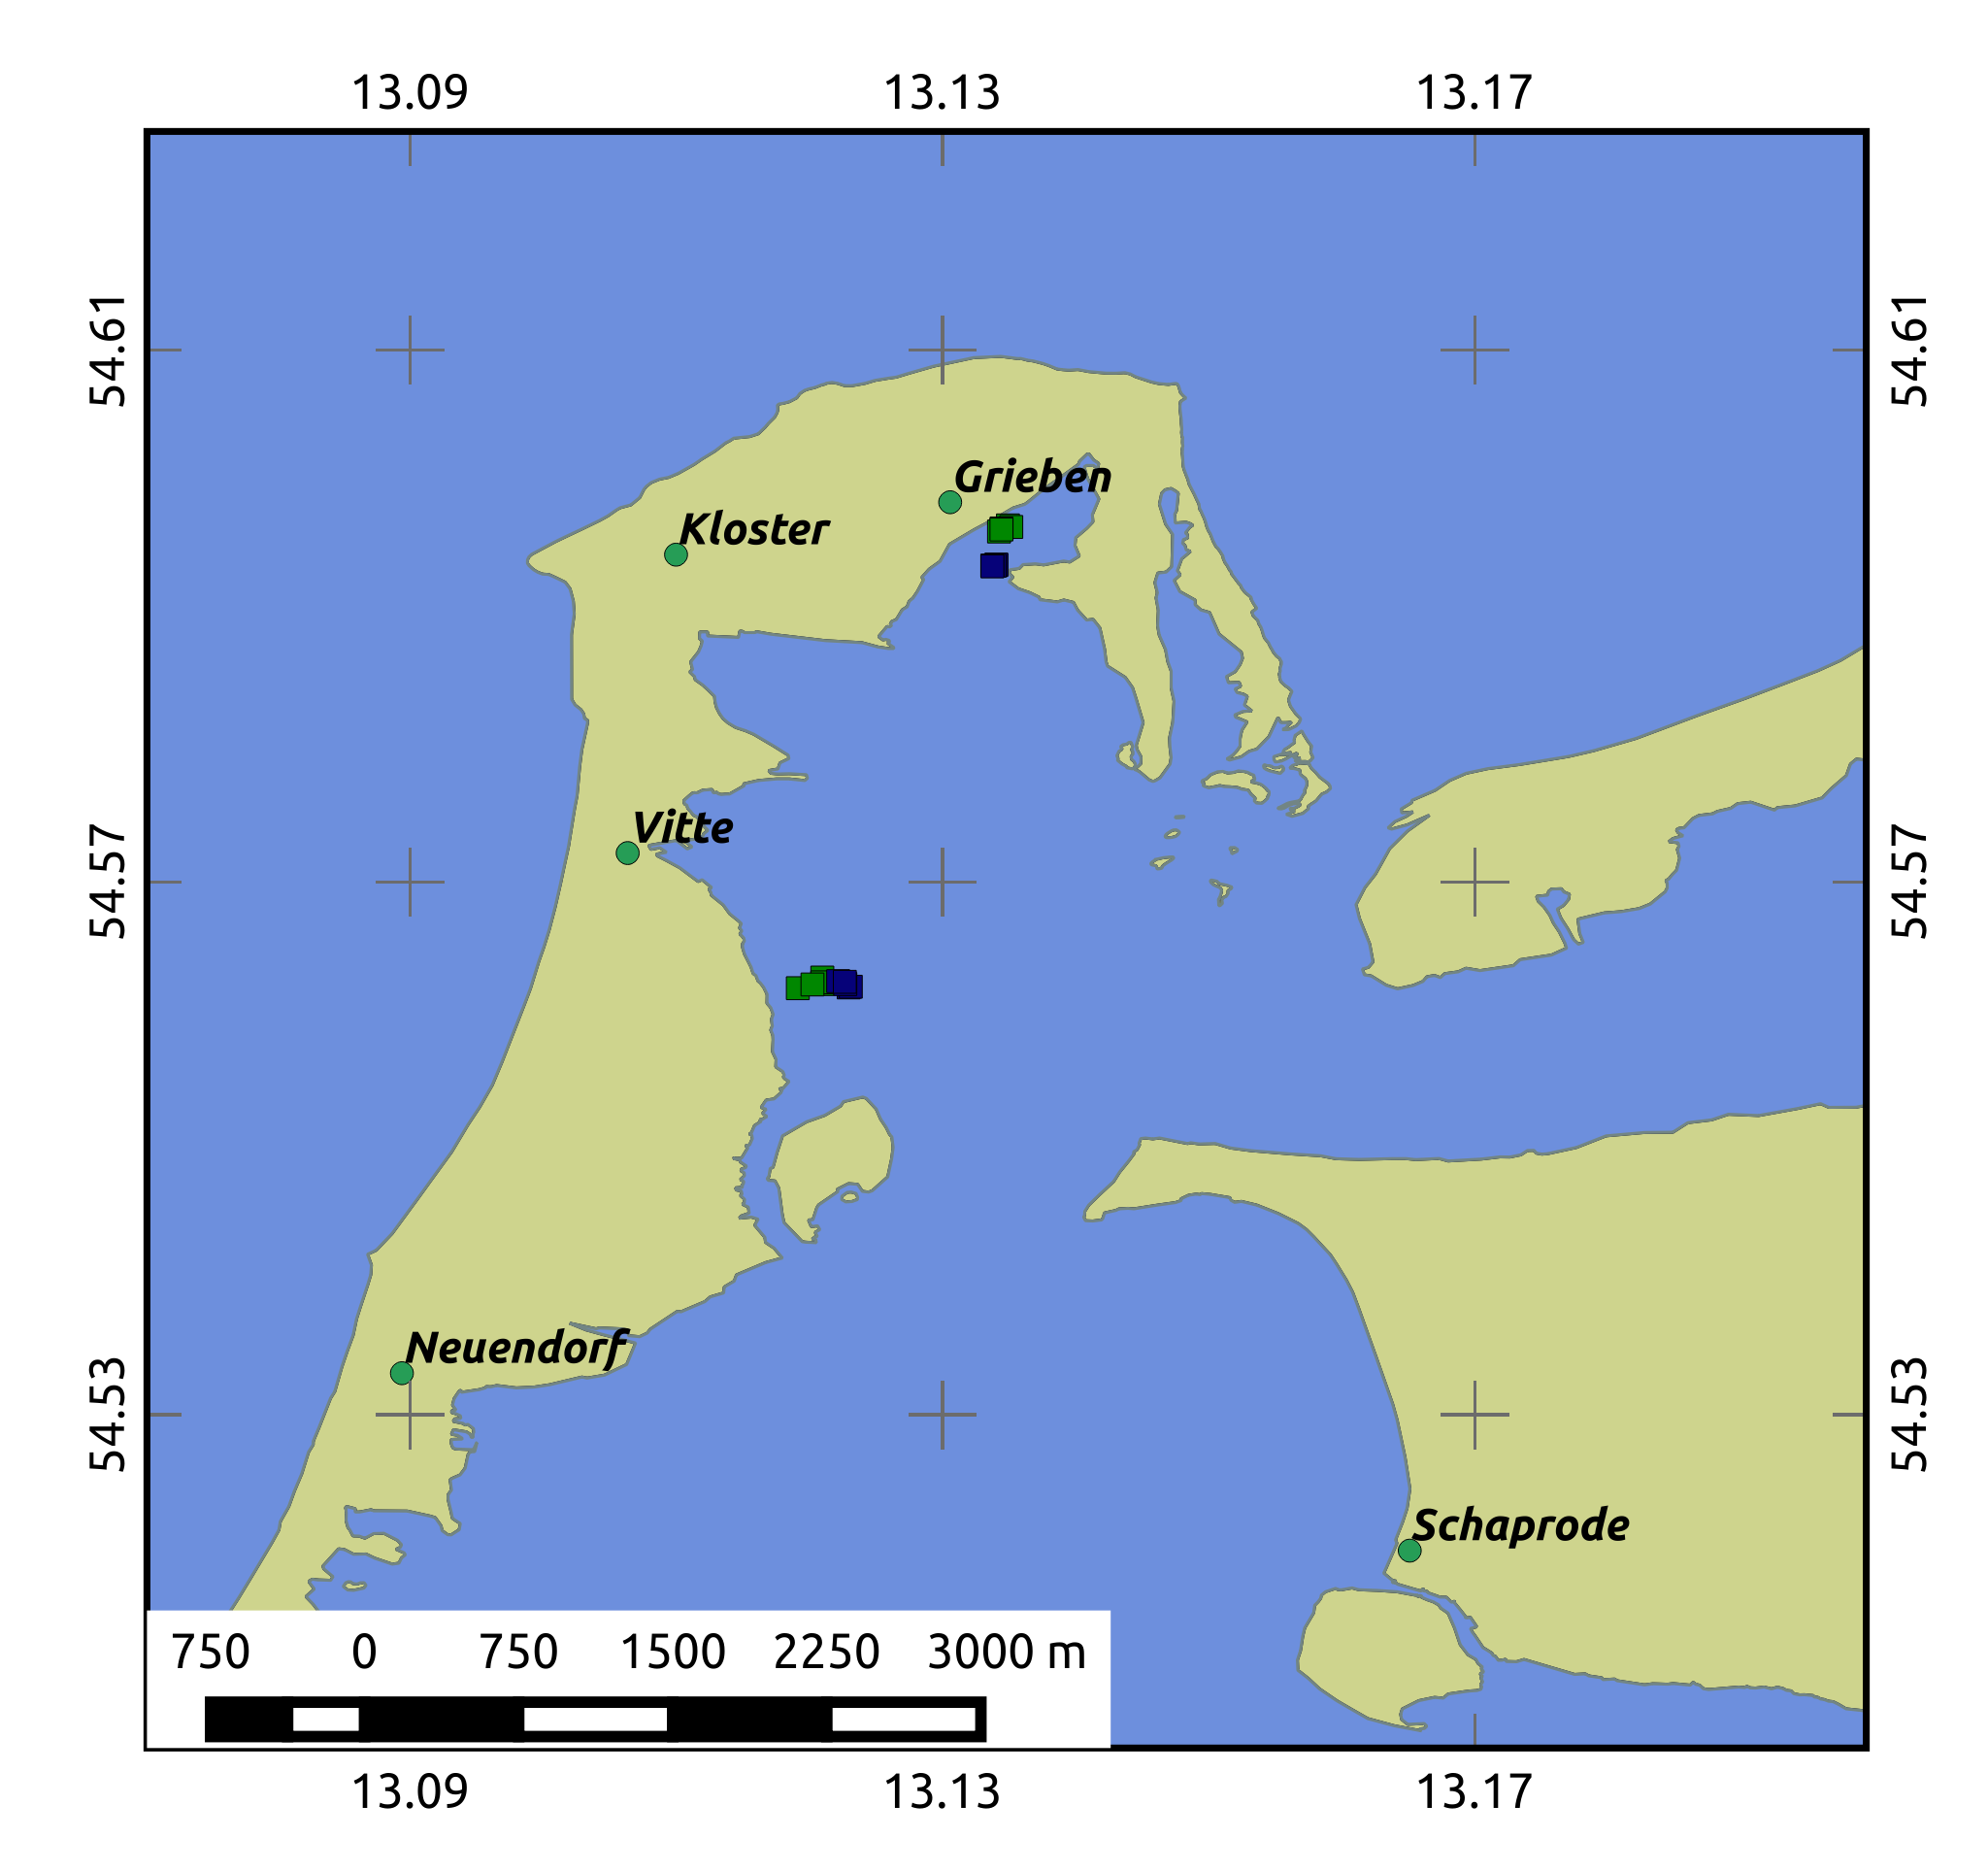
\includegraphics[height=0.8\textheight]{images/Hiddensee.png}
\end{figure}
\end{frame}

\begin{frame}
\frametitle{Vitte}
\begin{columns}
\begin{column}{7.5cm}
\begin{figure}
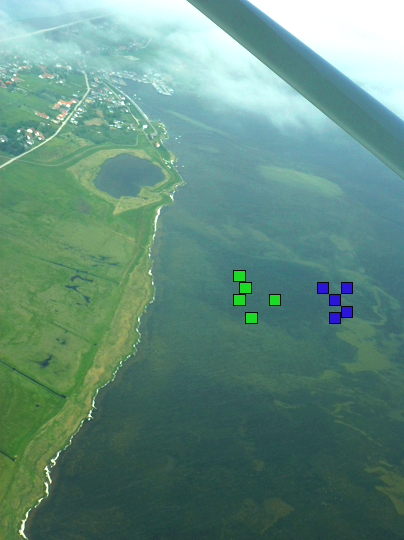
\includegraphics[height=0.8\textheight]{images/Fotos/vitte.png}
\end{figure}
\end{column}
\begin{column}{4cm}
\begin{itemize}
\item[\textcolor{green}{$\blacksquare$}] Flächen mit dichter Vegetation
\item[$ \hookrightarrow $] 0,8m tief
\item[]
\item[\textcolor{blue}{$\blacksquare$}] Flächen mit spärlicher Vegetation 
\item[$ \hookrightarrow $] 0,6m tief
\end{itemize}
\end{column}
\end{columns}
\end{frame}

\begin{frame}
\frametitle{Grieben}
\begin{columns}
\begin{column}{7.5cm}
\begin{figure}
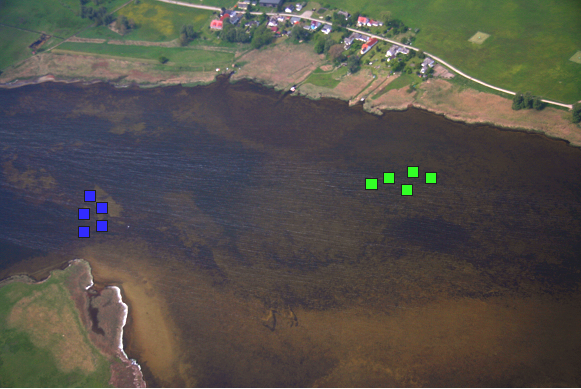
\includegraphics[width=\textwidth]{images/Fotos/griebenerbucht.png}
\end{figure}
\end{column}
\begin{column}{4cm}
\begin{itemize}
\item[\textcolor{green}{$\blacksquare$}] Flächen mit dichter Vegetation
\item[$ \hookrightarrow $] 0,8-0,9m tief
\item[]
\item[\textcolor{blue}{$\blacksquare$}] Flächen mit spärlicher Vegetation 
\item[$ \hookrightarrow $] 0,6-0,7m tief
\end{itemize}
\end{column}
\end{columns}
\end{frame}

\section{Methoden}
\subsection{Vegetation}

\begin{frame}
\frametitle{Vegetationskartierung}
\begin{columns}
\begin{column}{5.5cm}
\begin{figure}
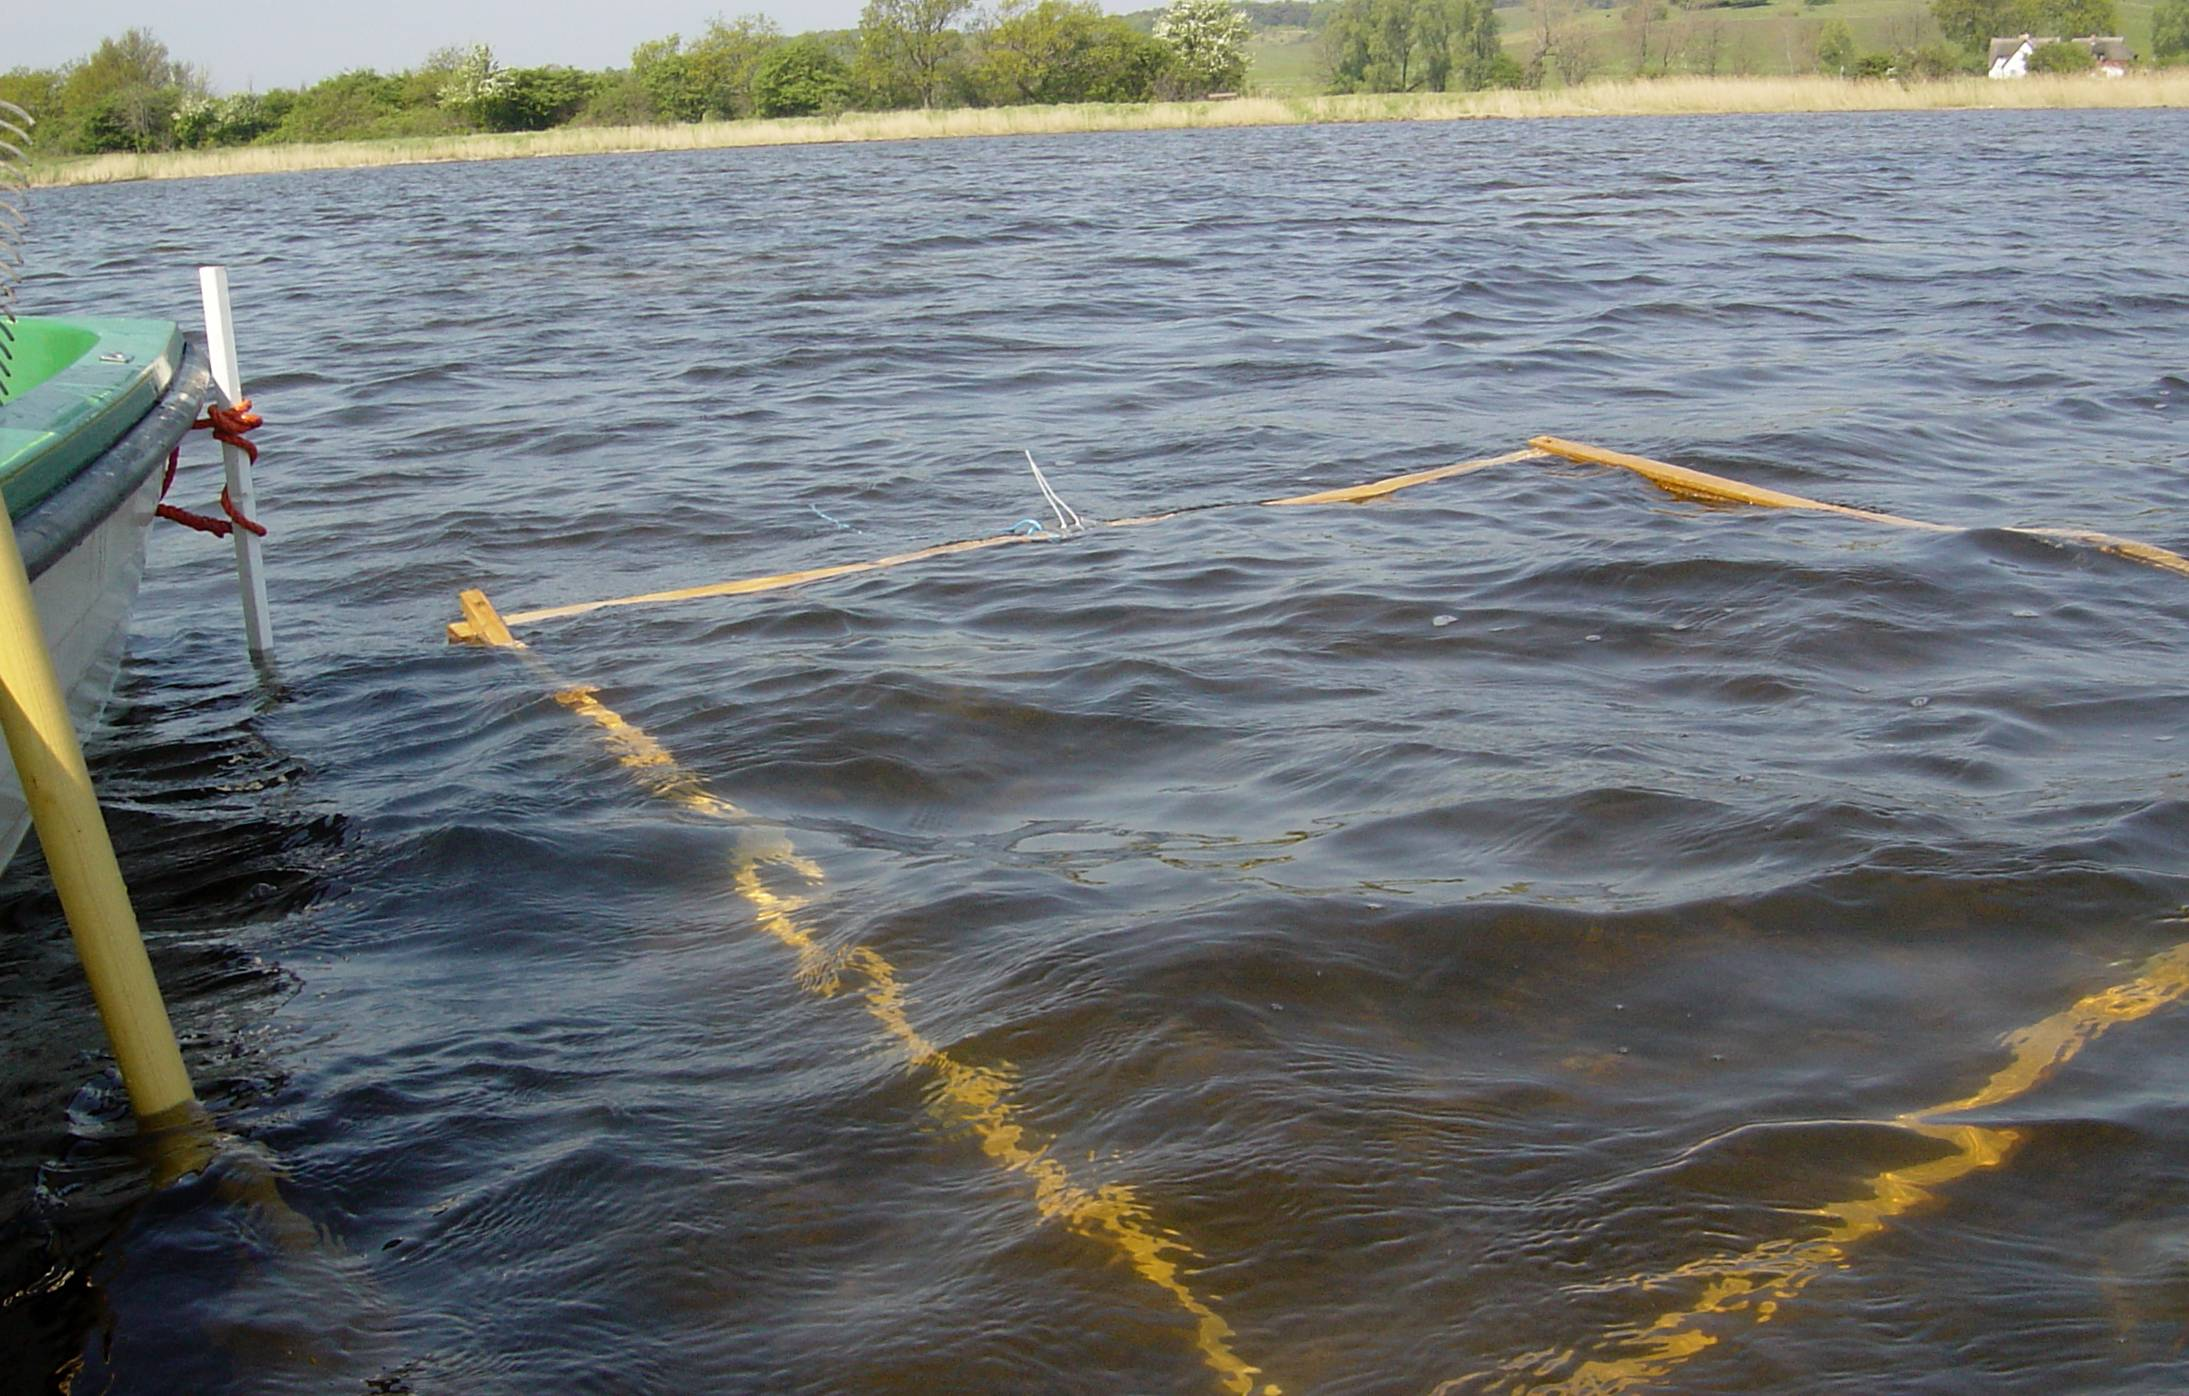
\includegraphics[height=35mm]{images/Fotos/vegetationsrahmen.jpg}
\end{figure}
\end{column}
\begin{column}{5.5cm}
\begin{figure}
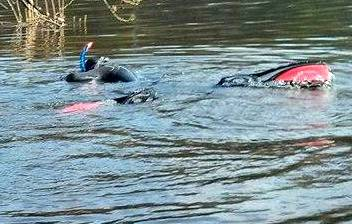
\includegraphics[height=35mm]{images/Fotos/schnorchelnklein2.jpg}
\vspace*{+5mm}
\end{figure}
\end{column}
\end{columns}
\end{frame}


\begin{frame}
\begin{columns}
\begin{column}{5.5cm}
\begin{block}{Absolute Deckung}
Deckungsgrade: 
1\%; 2\%; 5\%; 10\%; 20\%; 30\%; ... ; 100\% 
\end{block}
\begin{figure}
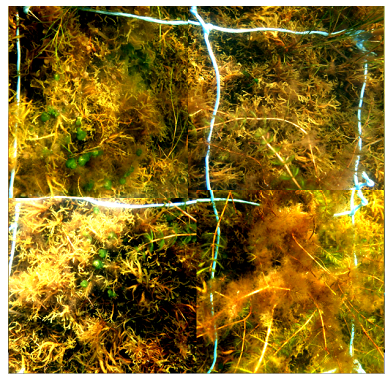
\includegraphics[height=40mm]{images/plotpictures/V+M.png}
\end{figure}
\end{column}
\visible<2>{
\begin{column}{5.5cm}
\begin{block}{Höhenstufenkartierung}
Höhenstufen: 
5cm; 10cm; 20cm; 30cm; 40cm ...
\end{block}
\begin{figure}
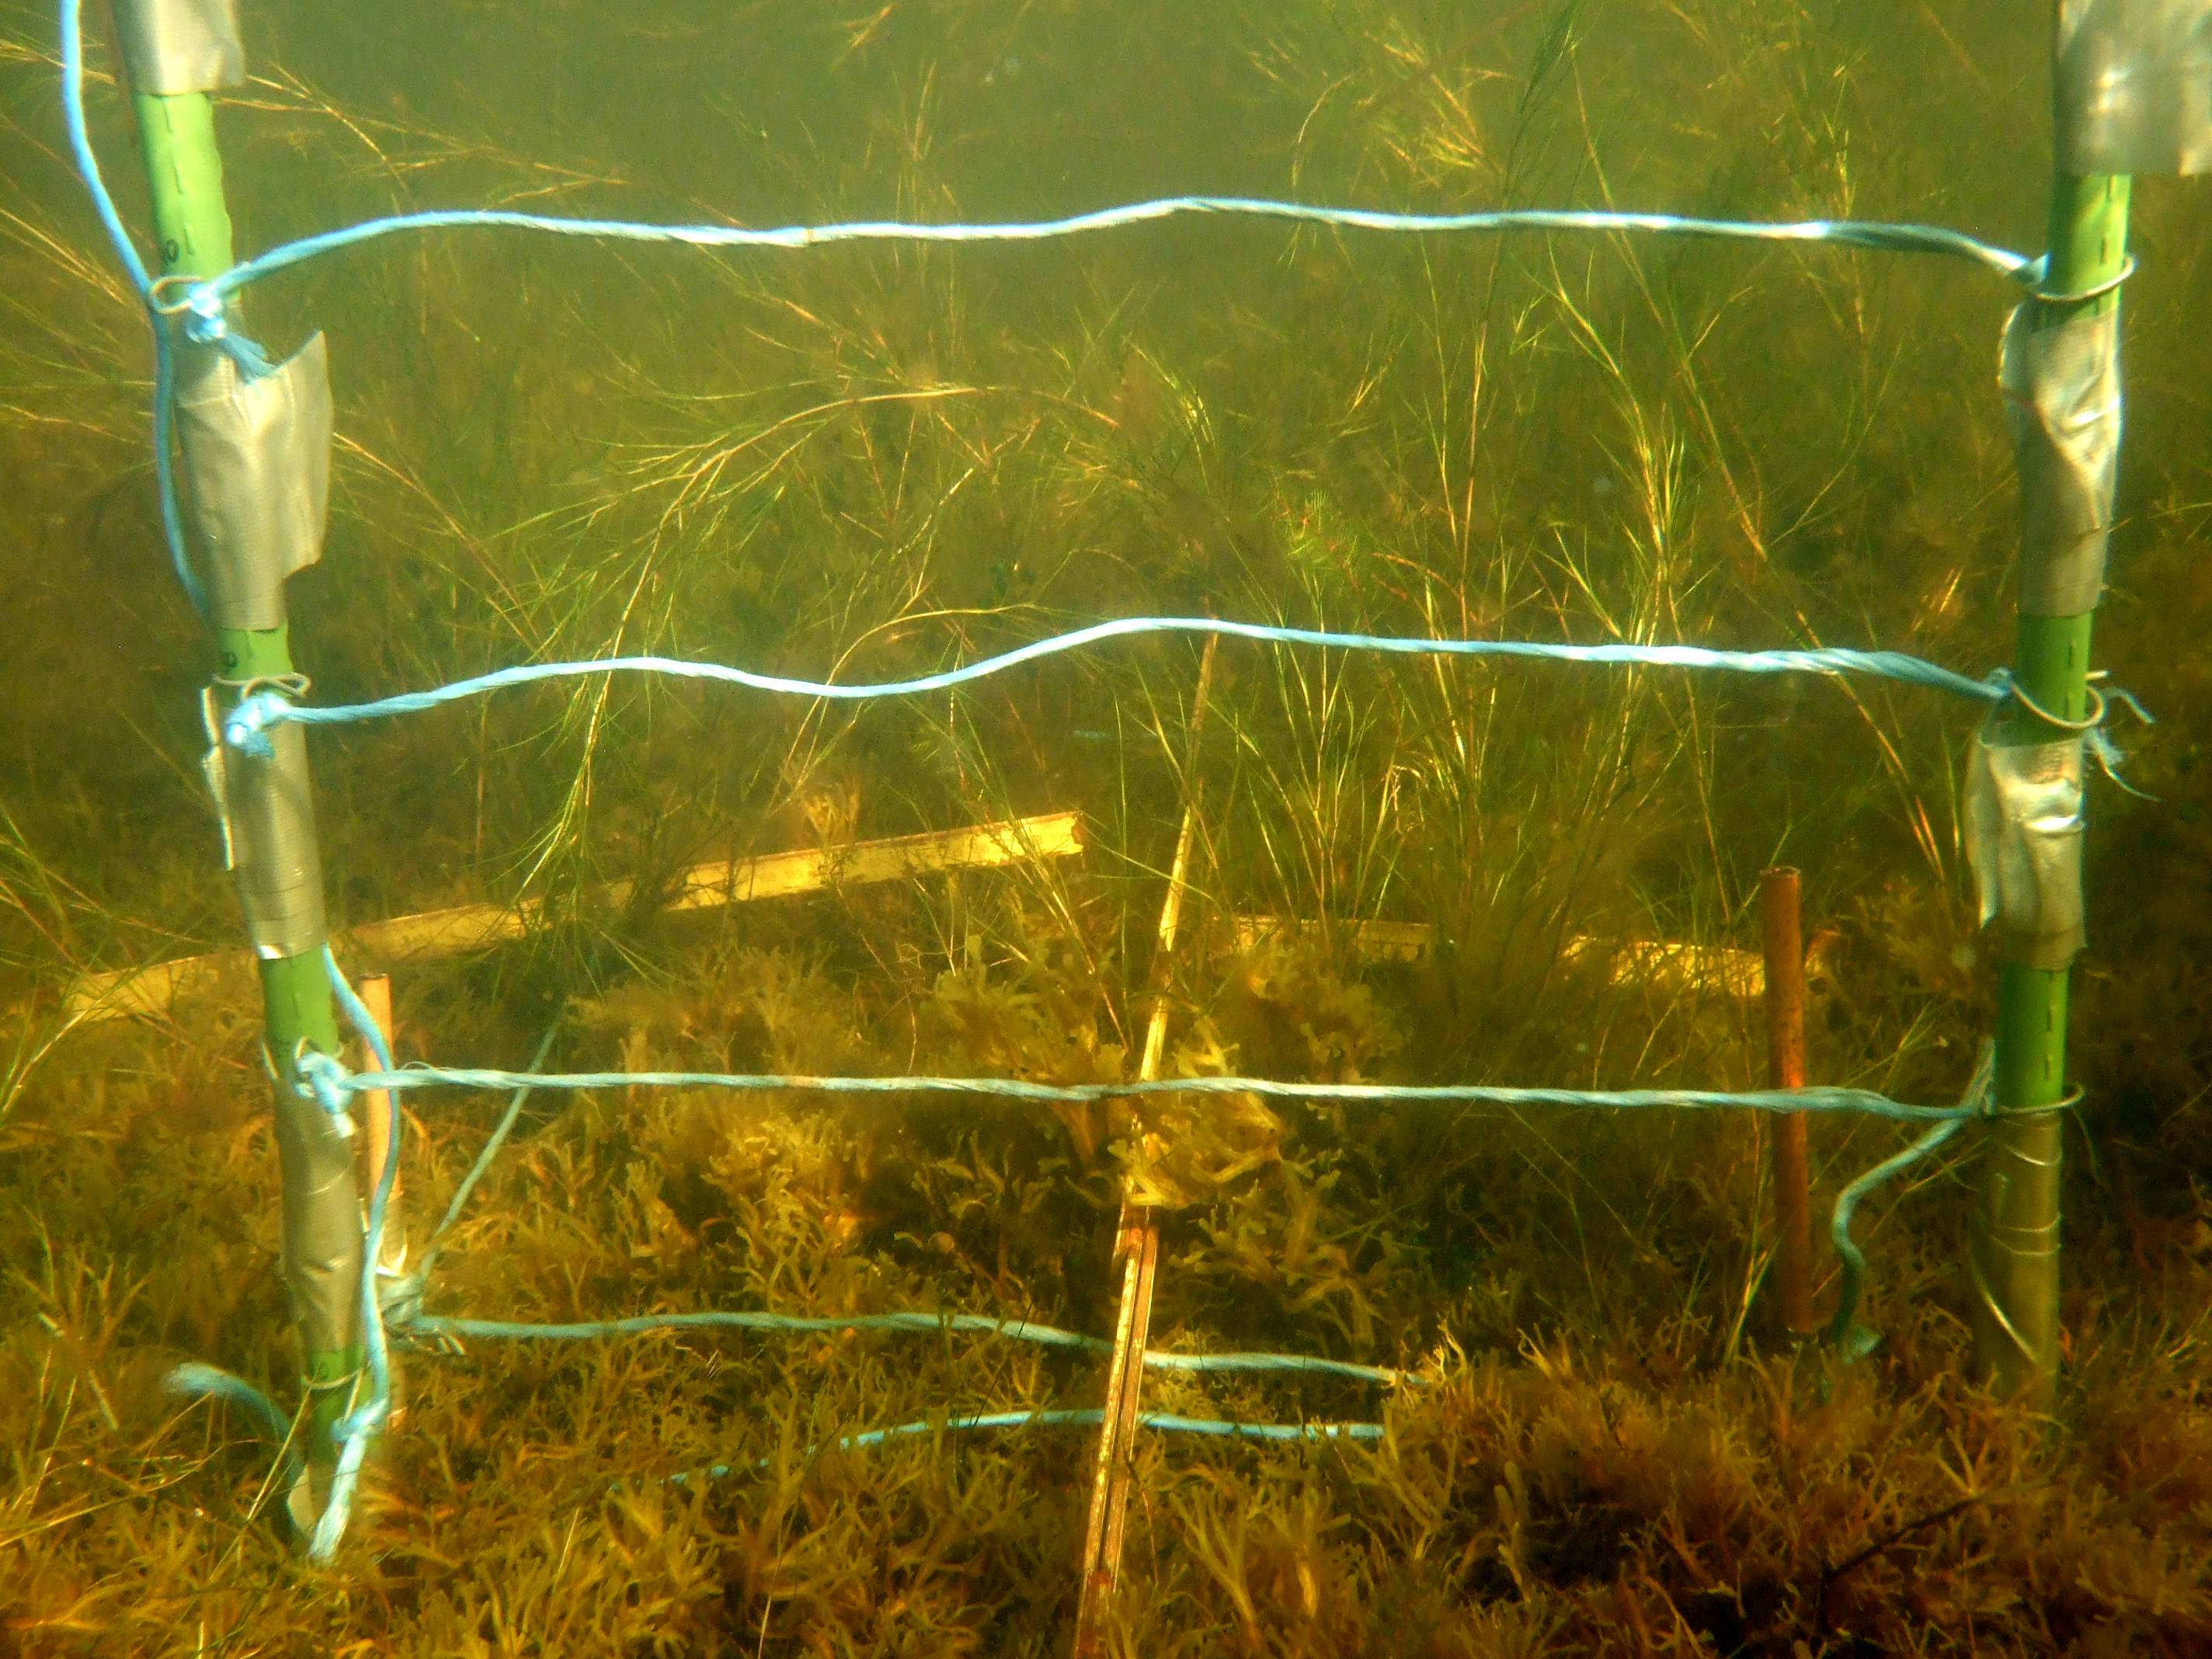
\includegraphics[height=40mm]{images/Fotos/DSCF0510.JPG}
\end{figure}
\end{column}}
\end{columns}
\end{frame}

\begin{frame}
\frametitle{Anteil der Pflanzen an der Wassersäule (PVI)}
\begin{block}{Berechnung}
\begin{align*}
 PVI &=\frac{\sum_{i=a}^n \frac{H_i * C_i}{100}}{\text{mittlere Wassertiefe}} & H_i &=\text{Länge einer jeden Höhenschicht}\\ 
 & & C_i &=\text{Deckung auf dieser Höhenschicht}\\
 & & a-n &=\text{Höhenstufen vom Boden}\\
 & &     &\text{\quad bis zur Wasseroberfläche}\\
\end{align*}
\end{block}
\end{frame}

\subsection{Sediment}
\begin{frame}
\frametitle{Sediment-Probenahme}
\begin{columns}
\begin{column}{6.4cm}
\begin{figure}
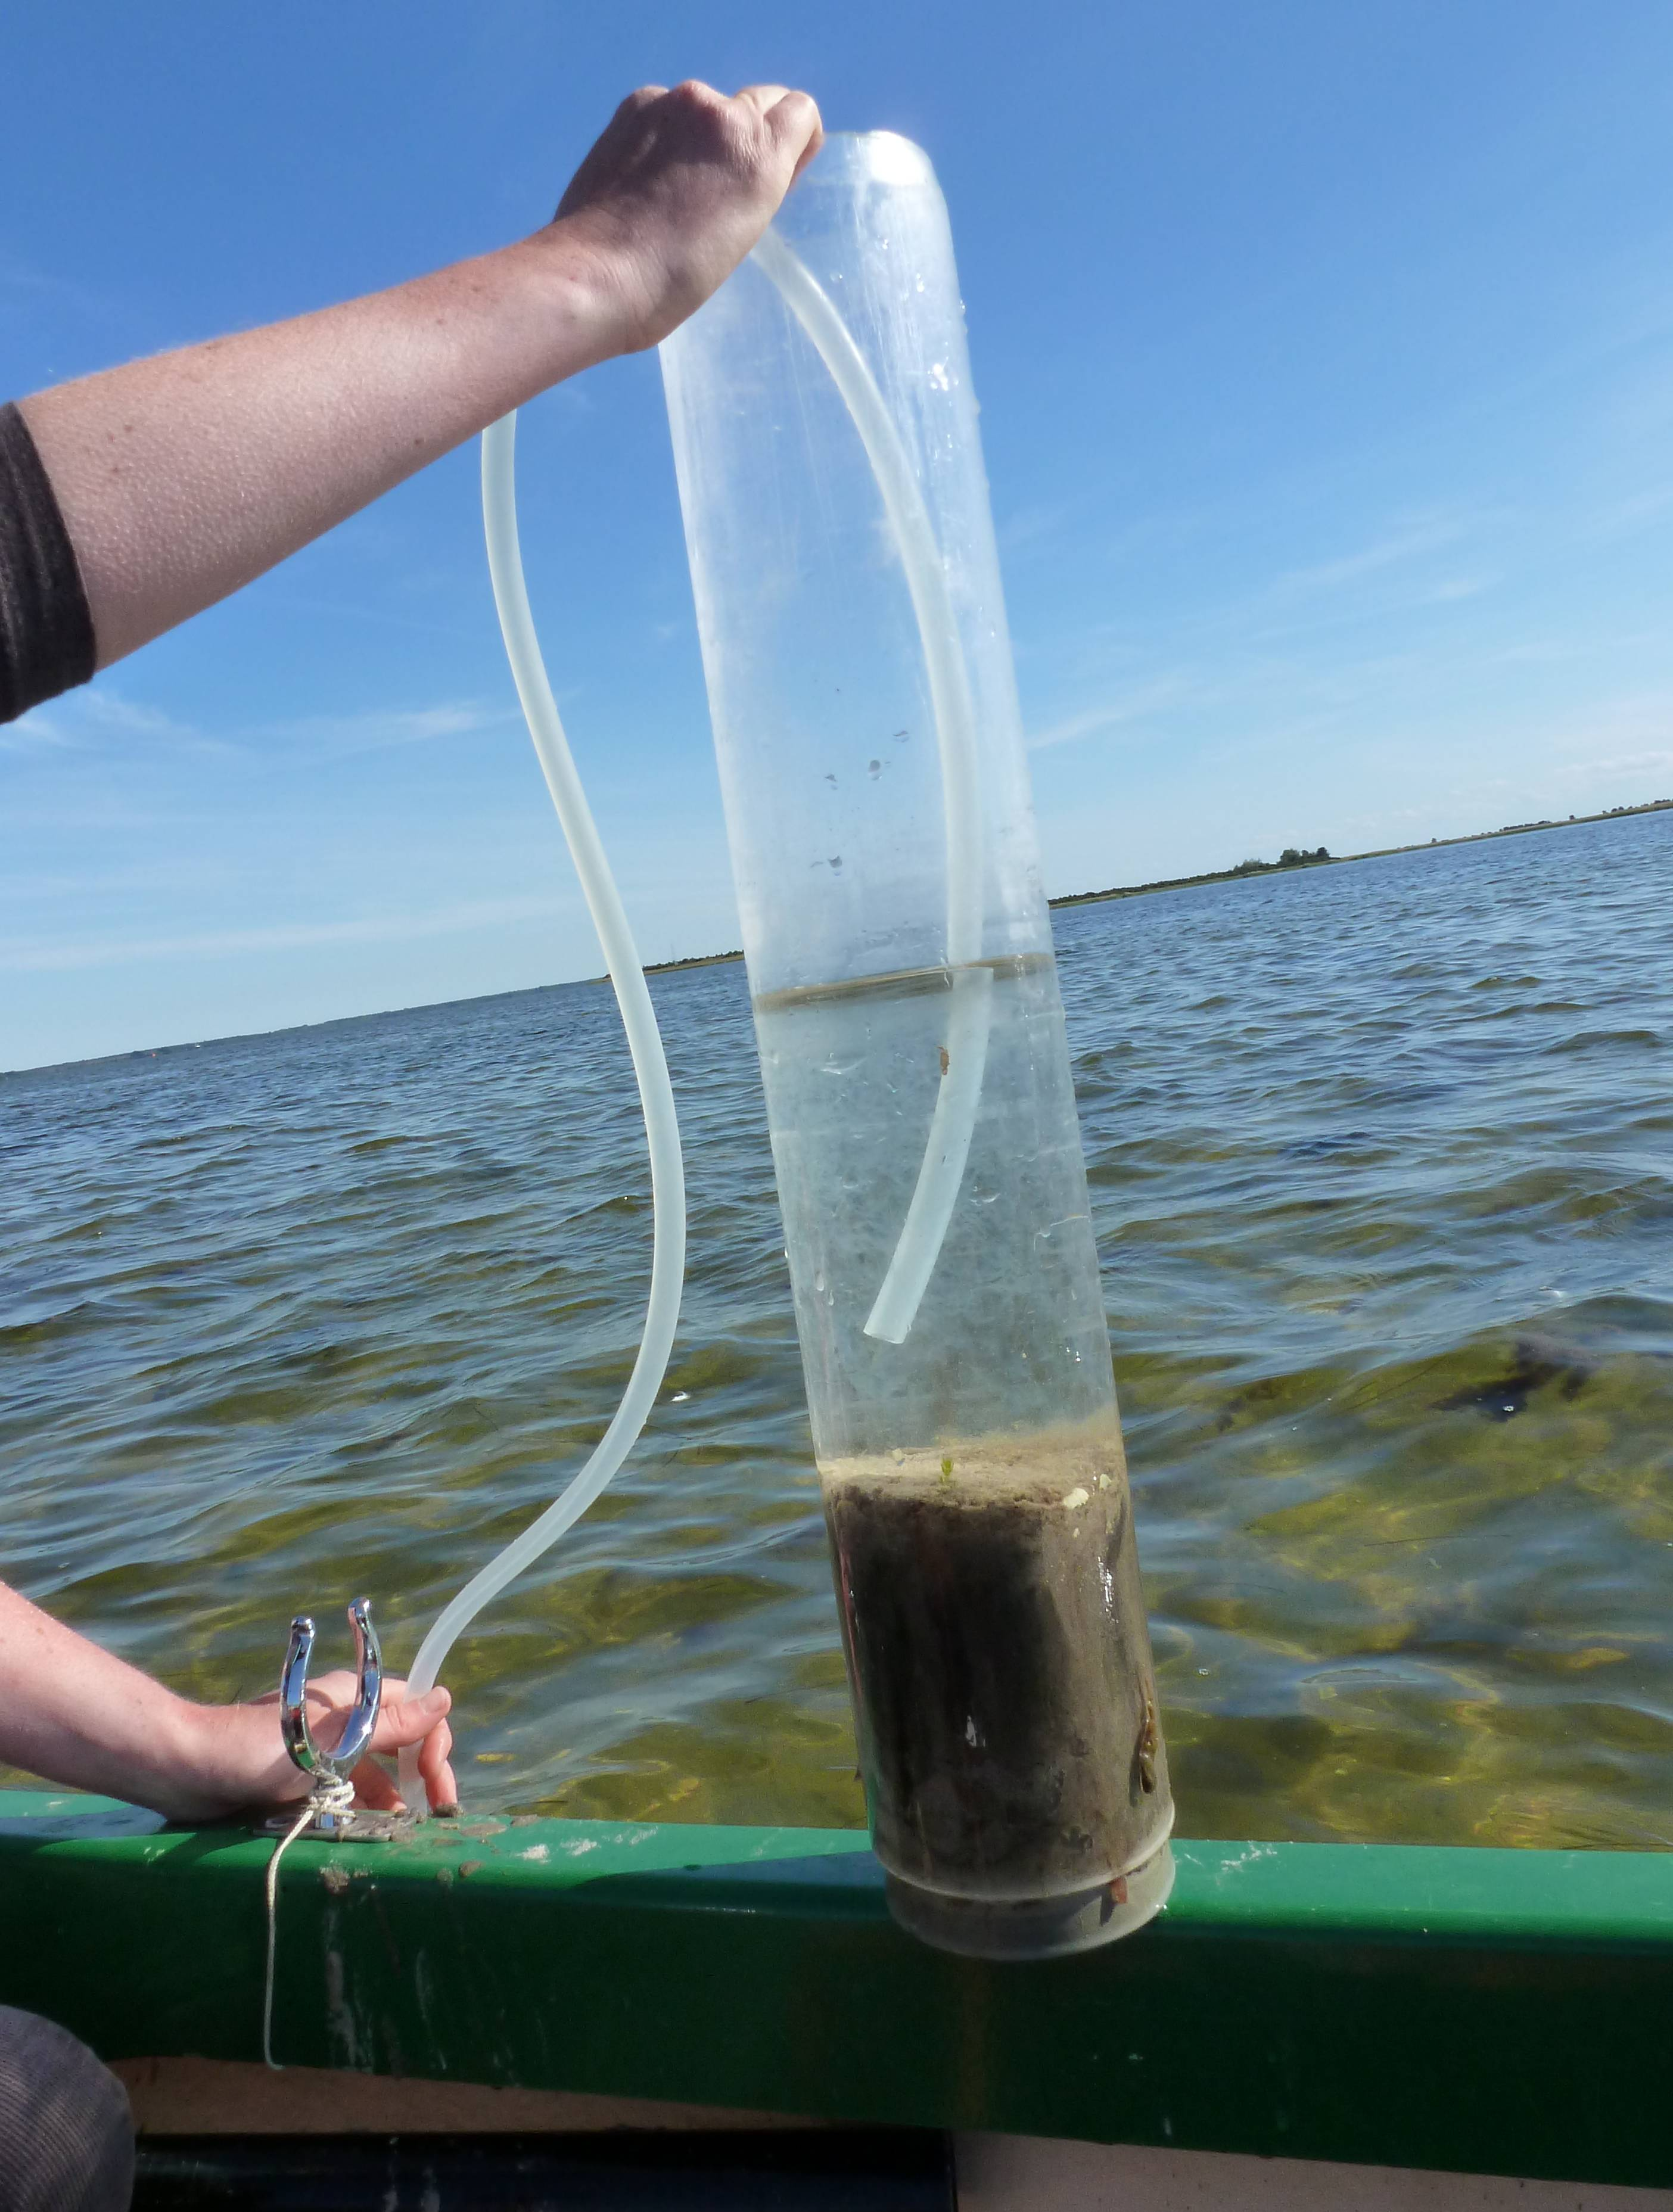
\includegraphics[height=55mm]{images/Fotos/Sedimentstechen.jpg}
\hspace*{-8mm}
\end{figure}
\end{column}
\begin{column}{6.4cm}
\begin{figure}
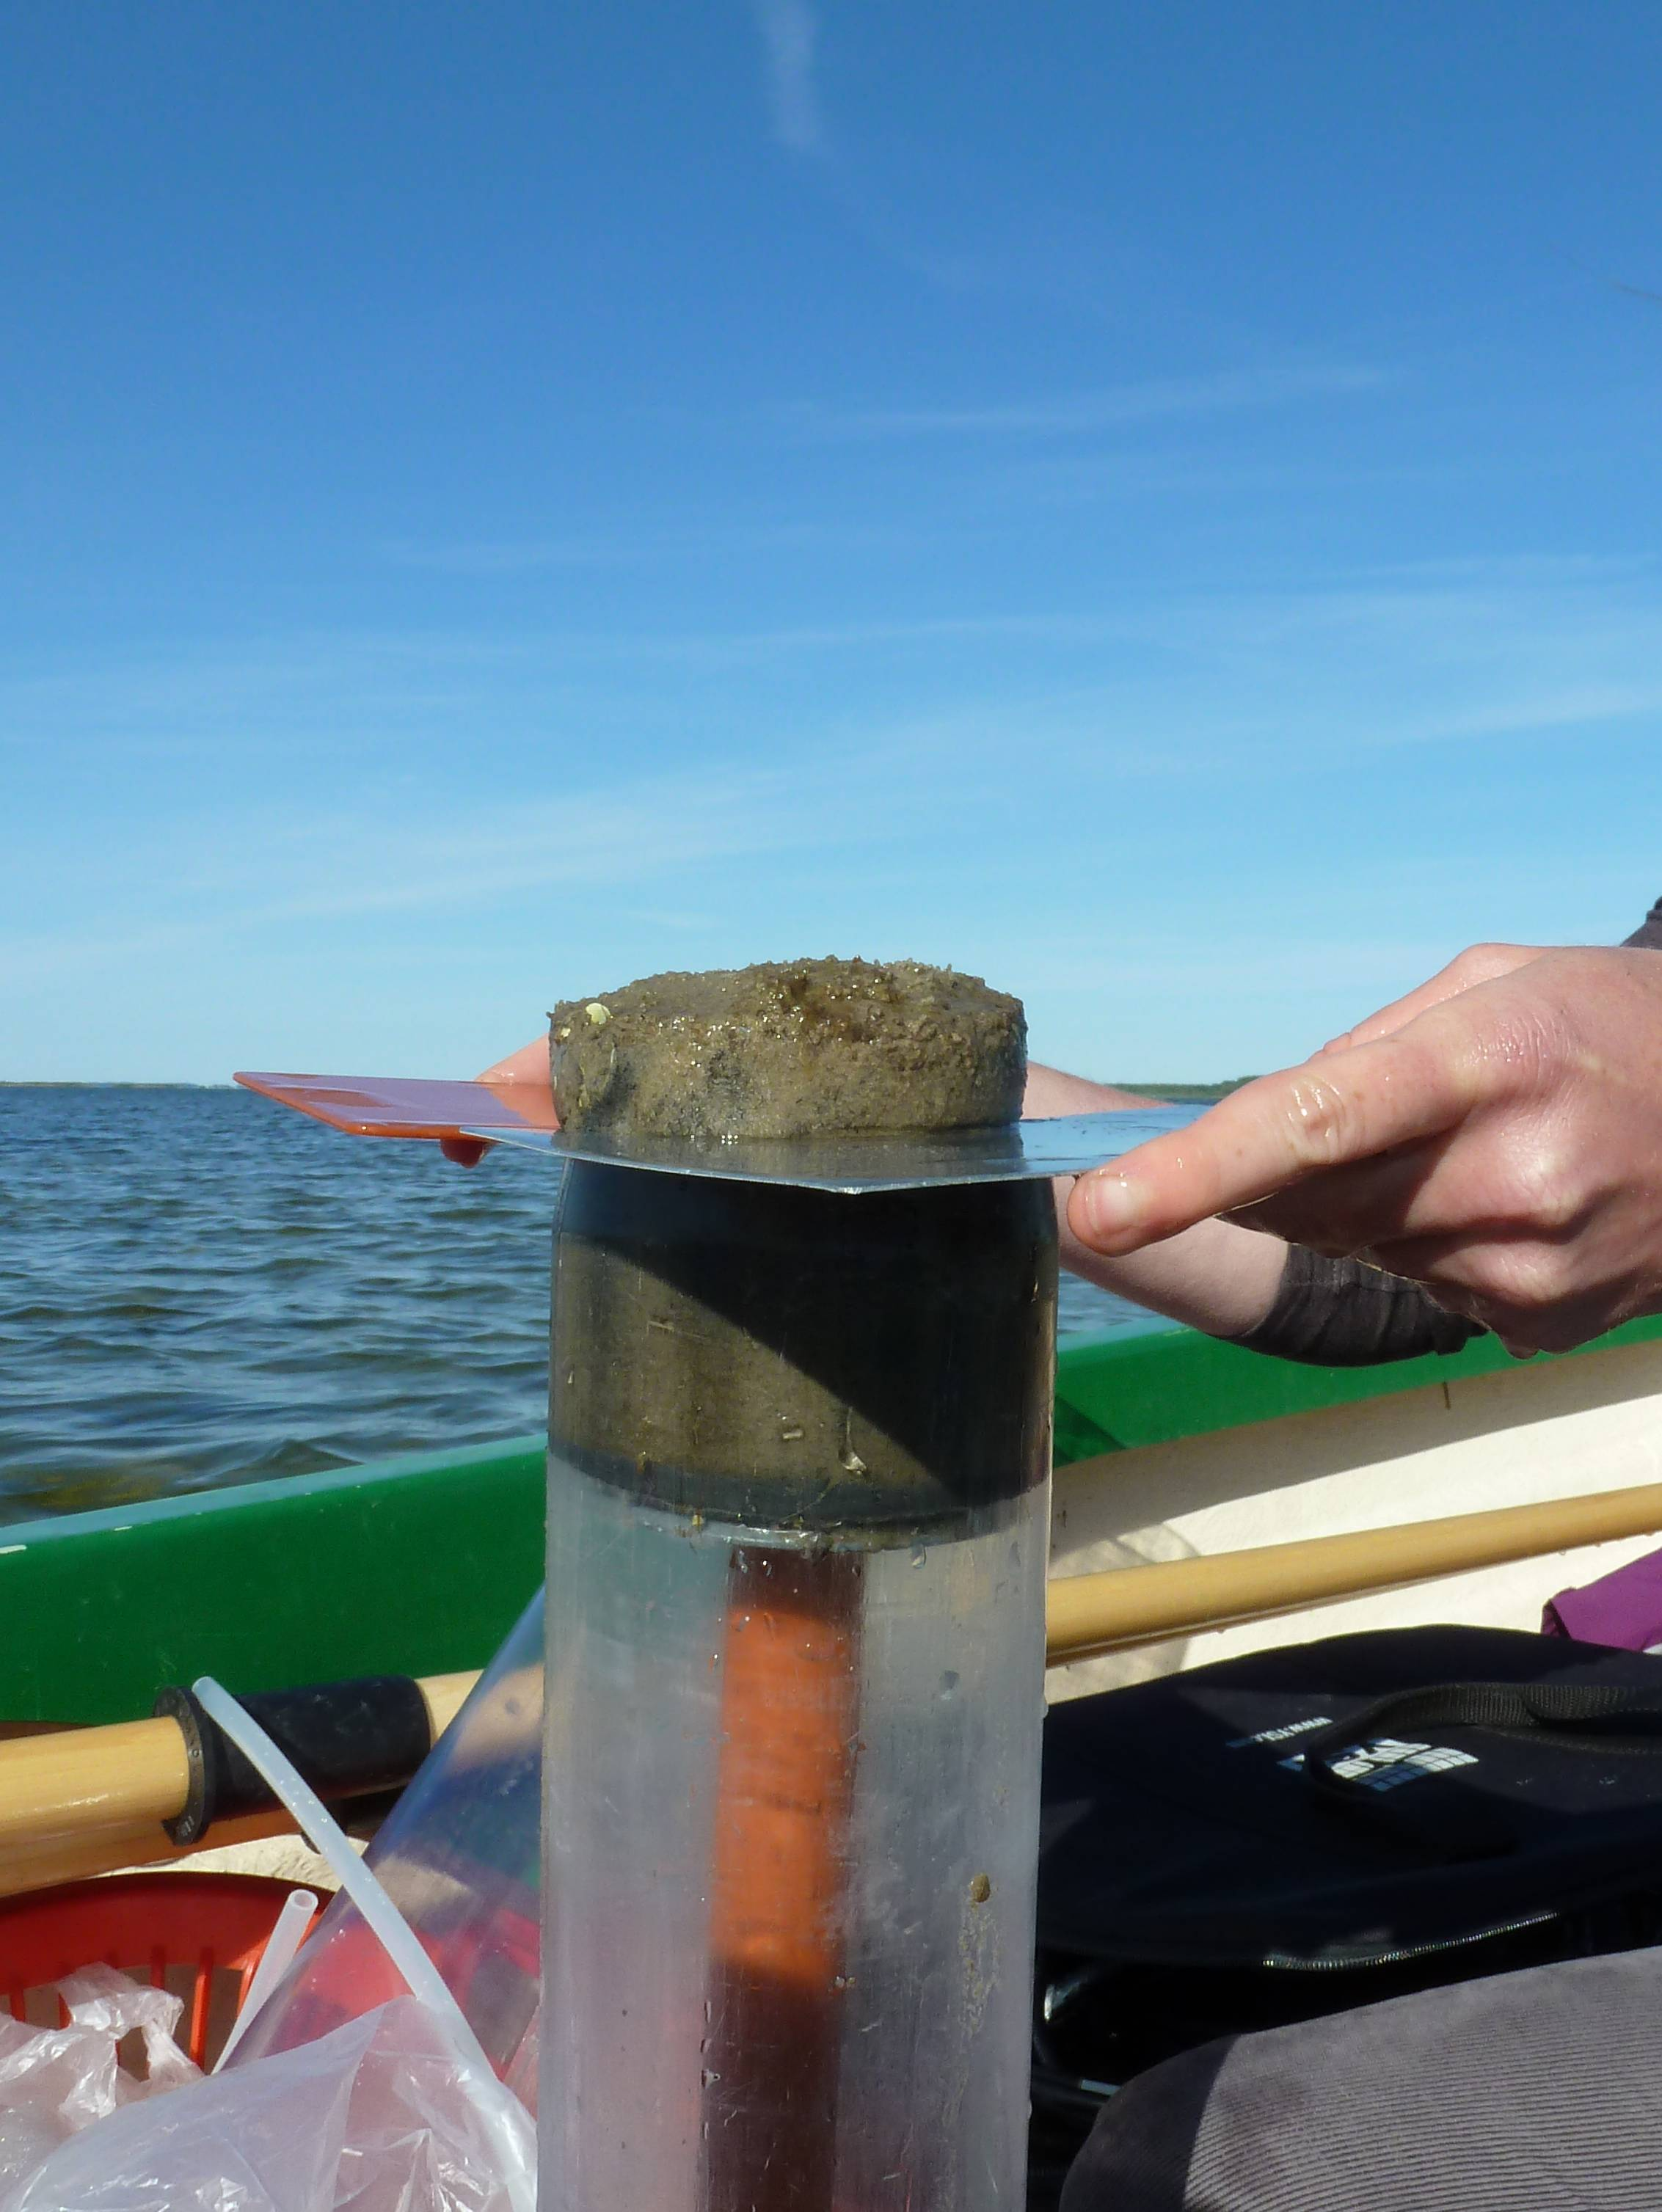
\includegraphics[height=55mm]{images/Fotos/Stempeln.jpg}
\hspace*{+8mm}
\end{figure}
\end{column}
\end{columns}
\end{frame}

\begin{frame}[t]
\frametitle{Korngrößenanalyse}
\begin{columns}[t]
\begin{column}{6.4cm}
\begin{figure}
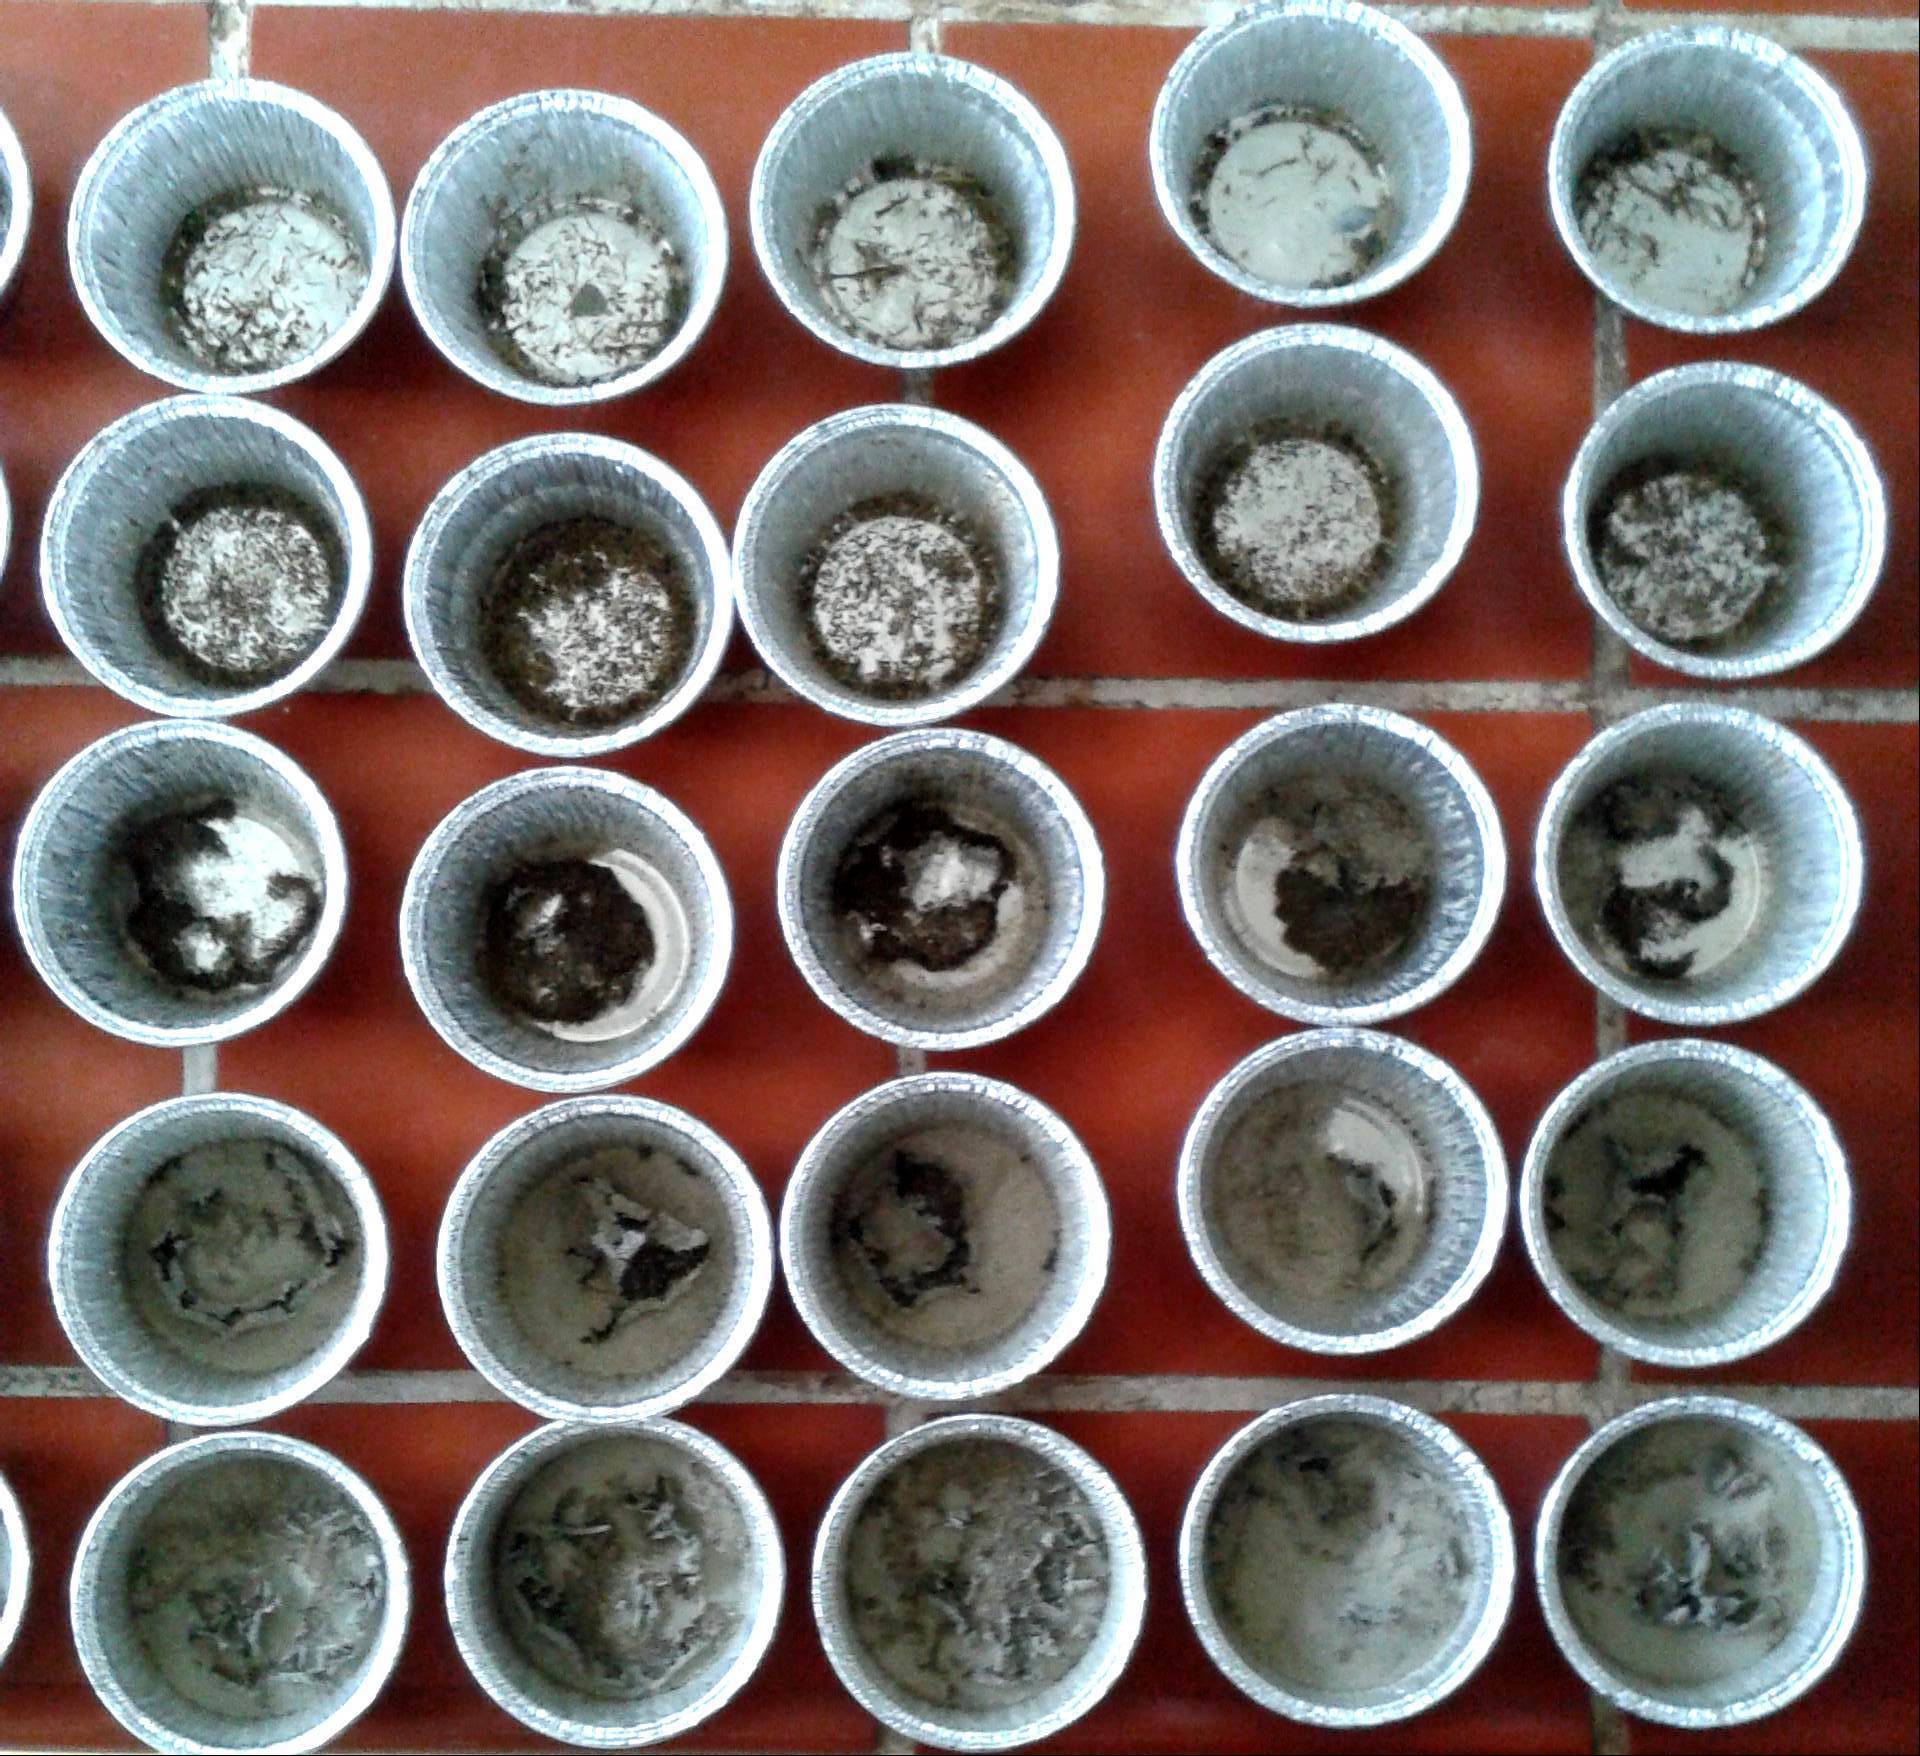
\includegraphics[width=0.8\textwidth]{images/Fotos/sediment.jpg} 

{\small Foto: Jutta Meyer}
\hspace*{-8mm}
\end{figure}
\end{column}

\begin{column}{4.4cm}
{\large Korngrößenfraktionen:}
\begin{itemize}
\item[]
\item[$\Phi = 0$]  sehr grober Sand
\item[$\Phi = 1$]  grober Sand
\item[$\Phi = 2$]  Mittelsand
\item[$\Phi = 3$]  feiner Sand
\item[$\Phi = 4$] sehr feiner Sand
\item[$\Phi = 5$] Ton und Schluff (berechnet)
\end{itemize}

\end{column}
\end{columns}
\end{frame}

%\subsection{Statistik}

%\begin{frame}[t]
%\frametitle{Statistische Auswertung}
%\begin{figure}
%\begin{flushleft}
%Häufigkeit (\%)
%\end{flushleft}
%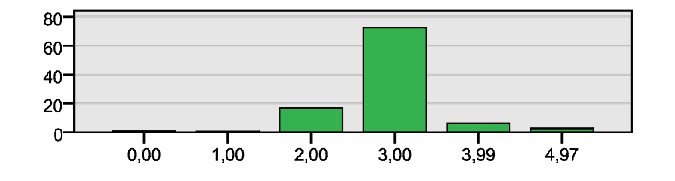
\includegraphics[height=30mm]{images/Fotos/bsp_kornverteilung.png}
%\vspace*{-0.76cm}
%\end{figure}
%\begin{flushright}
%Korngrößenklasse ($ \Phi $)
%\end{flushright}
%\begin{itemize}
%\setlength{\itemindent}{+5.5cm} 
%\item[Unterschiede zwischen $ +M $ und $ -M $:] Mann-Whithney-Test
%\item[Unterschiede im Jahresverlauf:] Kruskal-Wallis-Test, 
%\item[] Dunn's-Test 
%\end{itemize}
%\end{frame}


\section{Ergebnisse und Diskussion}
\subsection{Vegetation: Vitte}

\begin{frame}
\center
\textcolor{Blue}{{\LARGE Vegetation: Vitte}}
\end{frame}

\begin{frame}
\frametitle{Bedeckung mit Makrophytobenthos}
\begin{columns}
\begin{column}{6cm}
\begin{figure}
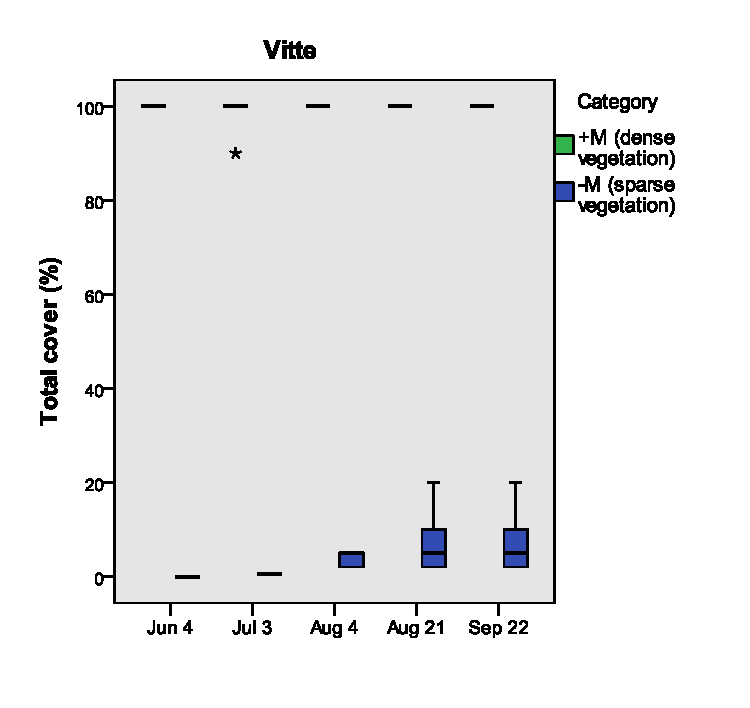
\includegraphics[width=\textwidth]{images/total_cover/total_cover1.eps}
\end{figure}
\end{column}
\begin{column}{6cm}
\begin{overprint}
\onslide<1>
\begin{figure}
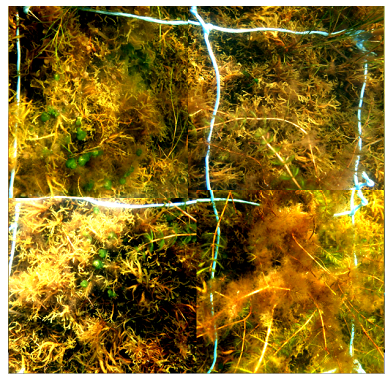
\includegraphics[width=\textwidth]{images/plotpictures/V+M.png}
\end{figure}

\onslide<2>
\begin{figure}
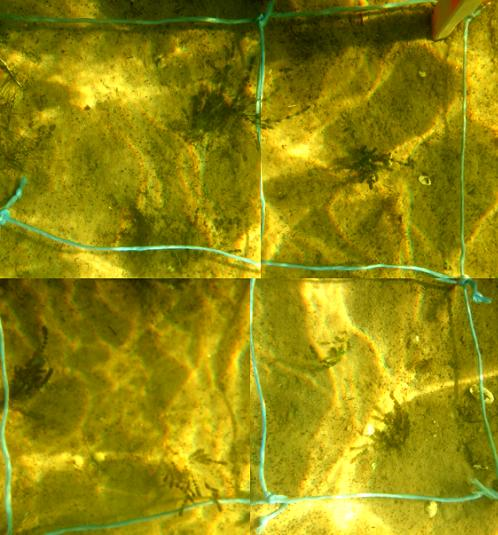
\includegraphics[width=\textwidth]{images/Fotos/vvonoben.jpg}
\end{figure}
\end{overprint}
\end{column}
\end{columns}
\end{frame}

\begin{frame}
\frametitle{PVI}
\begin{columns}
\begin{column}{7.0cm}
\begin{figure}
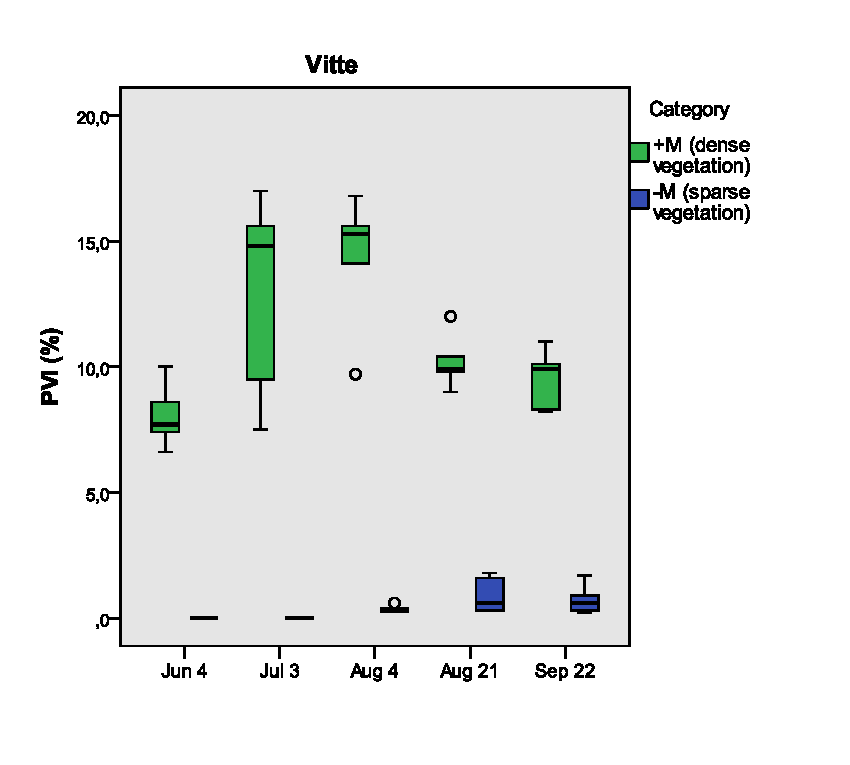
\includegraphics[width=\textwidth]{images/pvi/boxplot_pvi1.eps}
\hspace*{-9mm}
\end{figure}
\end{column}
\begin{column}{5.8cm}
\begin{figure}
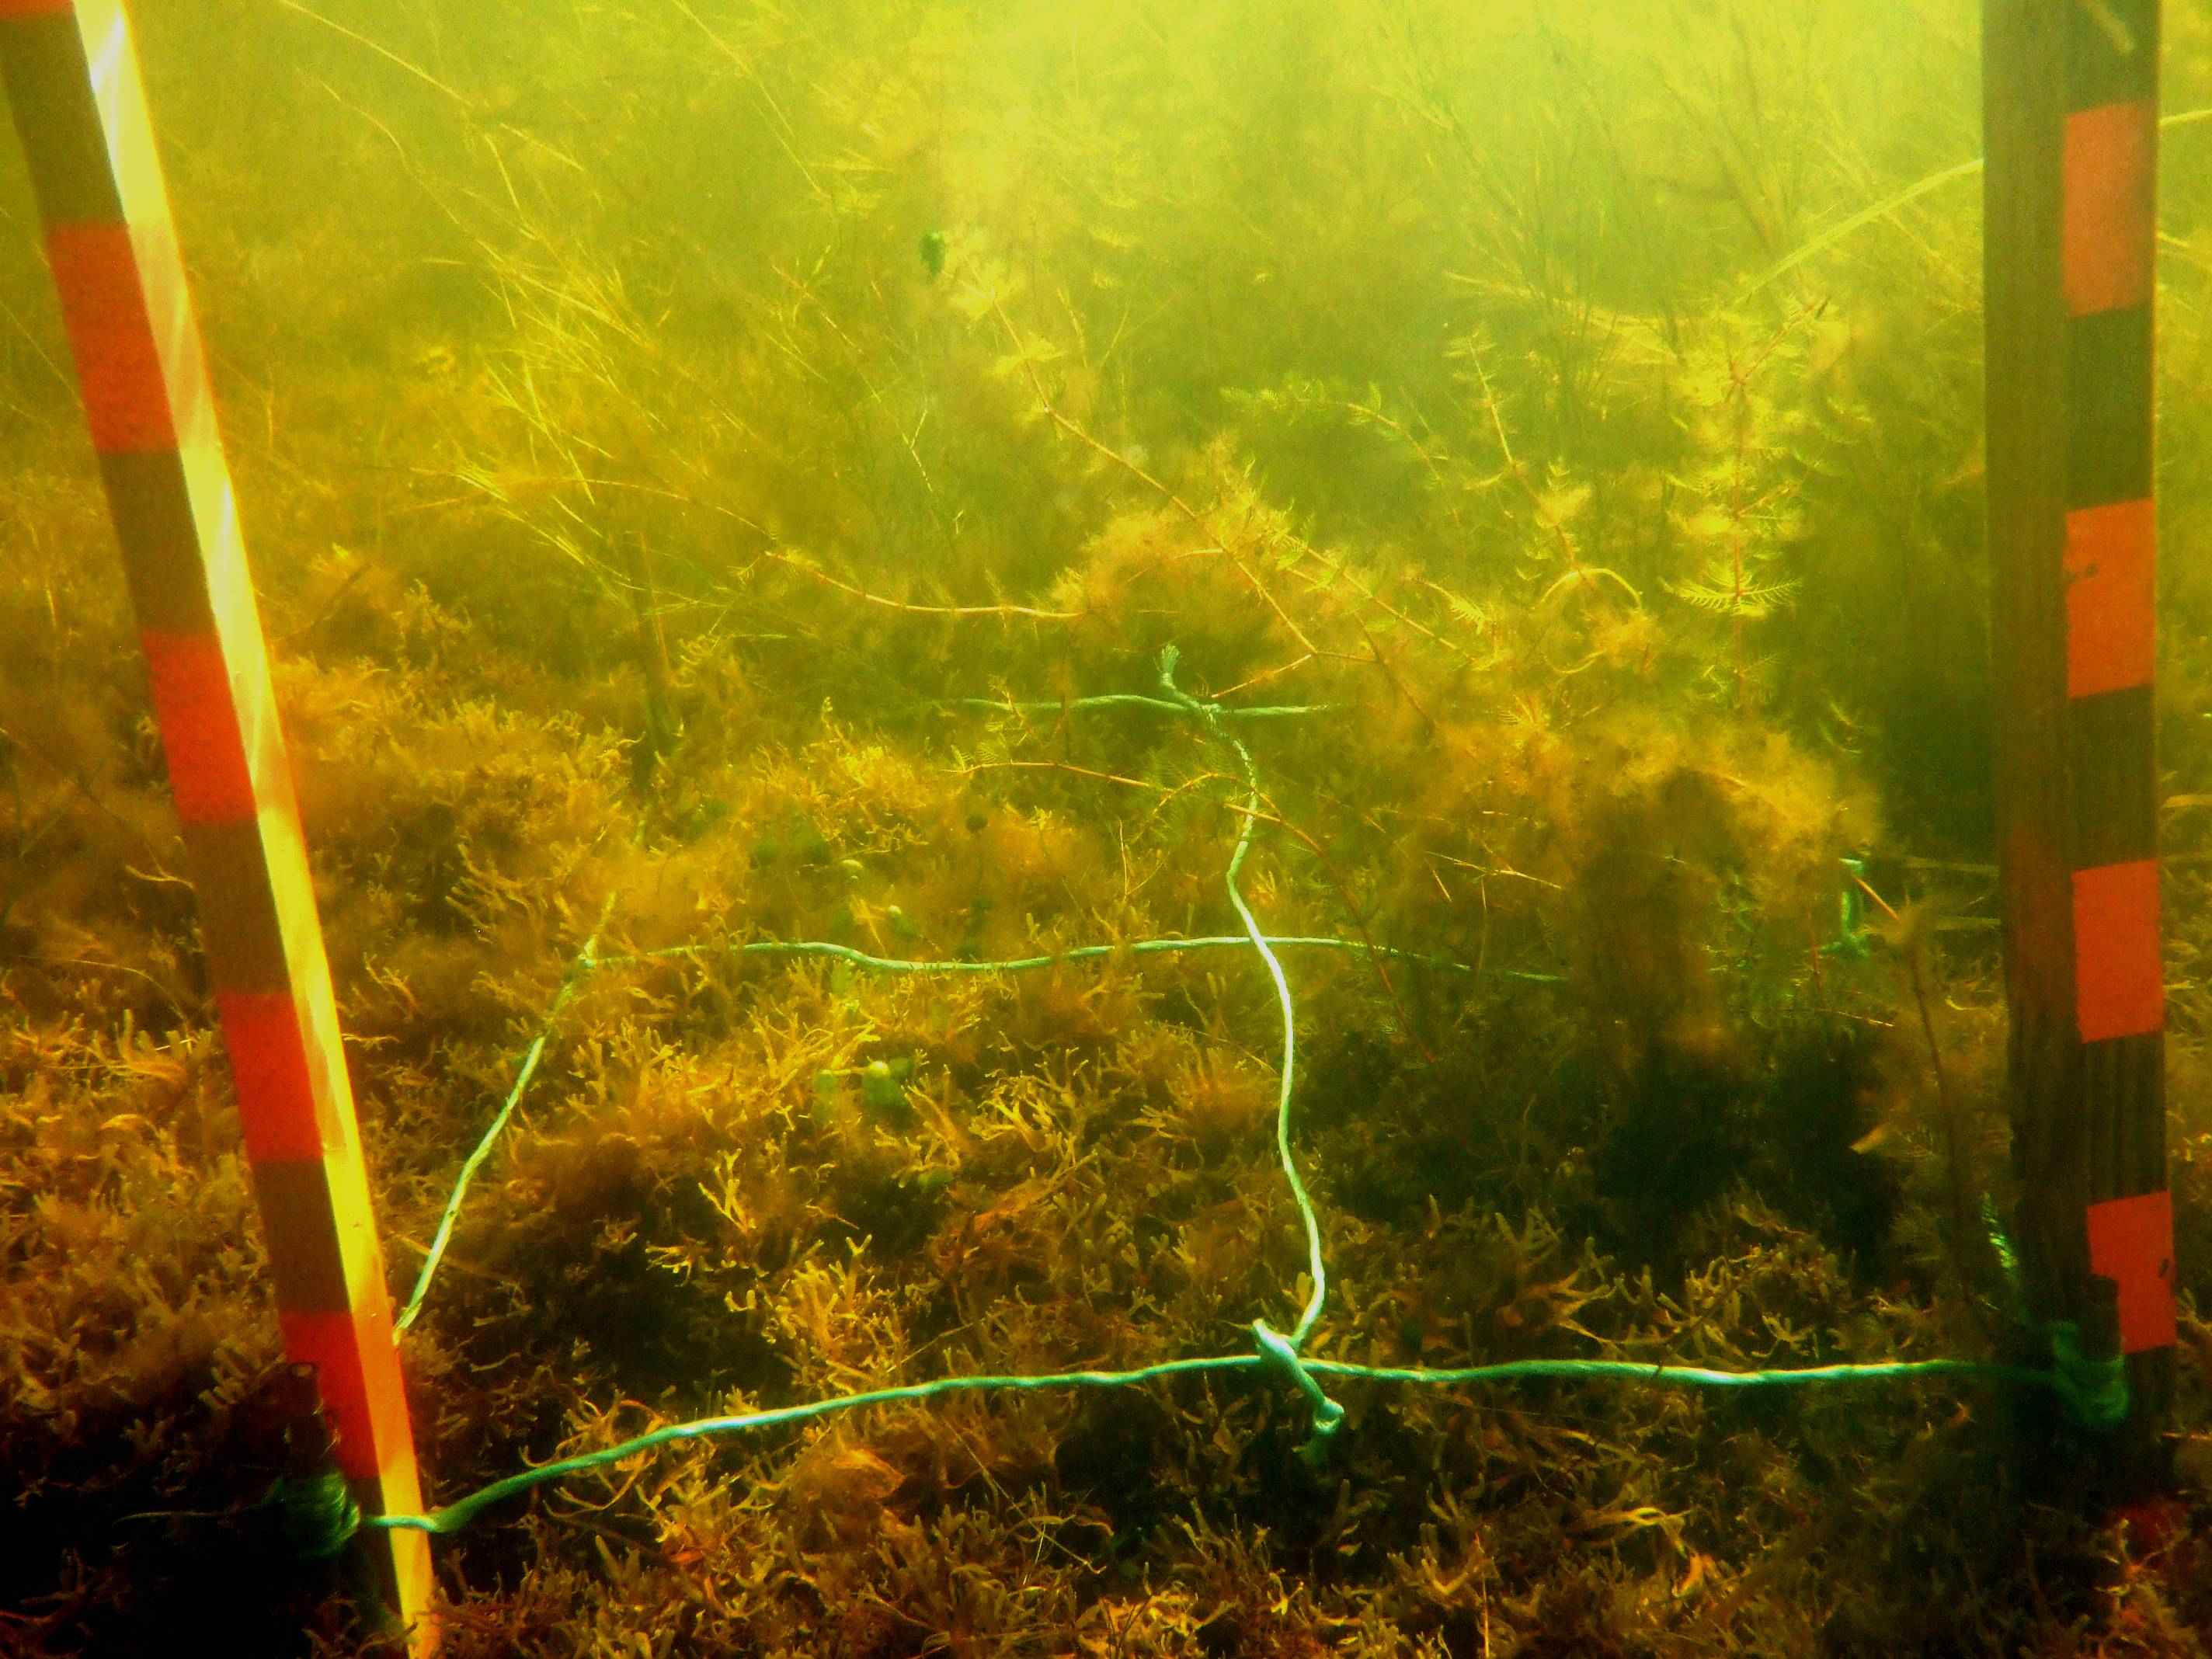
\includegraphics[width=0.9\textwidth]{images/plotpictures/BSP_V+M}
\hspace*{+8mm}
\end{figure}
\end{column}
\end{columns}
\end{frame}

\subsection{Vegetation: Grieben}
\begin{frame}
\center
\textcolor{Blue}{{\LARGE Vegetation: Grieben}}
\end{frame}

\begin{frame}
\frametitle{Bedeckung mit Makrophytobenthos}
\begin{columns}
\begin{column}{5.5cm}
\begin{figure}
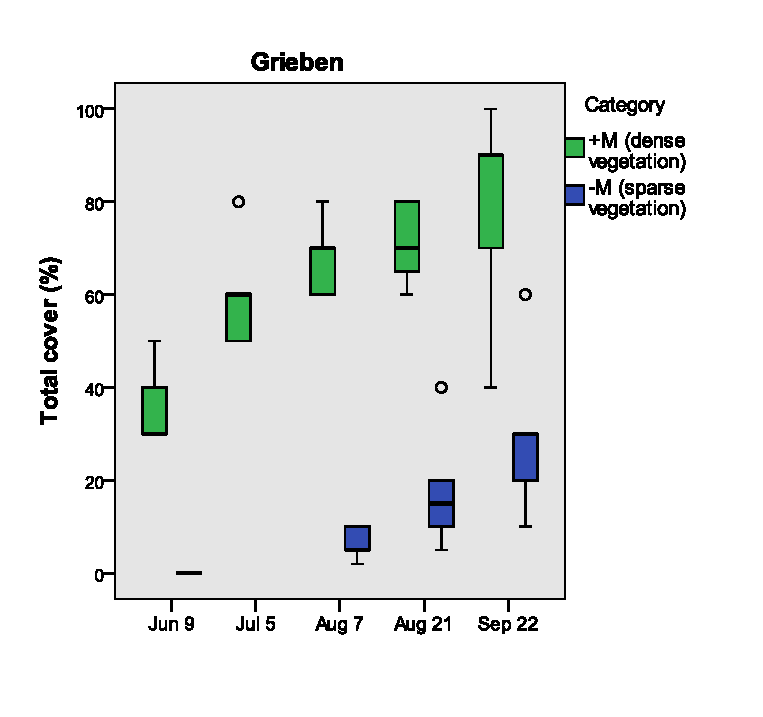
\includegraphics[width=\textwidth]{images/total_cover/total_cover2.eps}
\end{figure}
\end{column}
\begin{column}{5.5cm}
\begin{overprint}
\onslide<1>
\begin{figure}
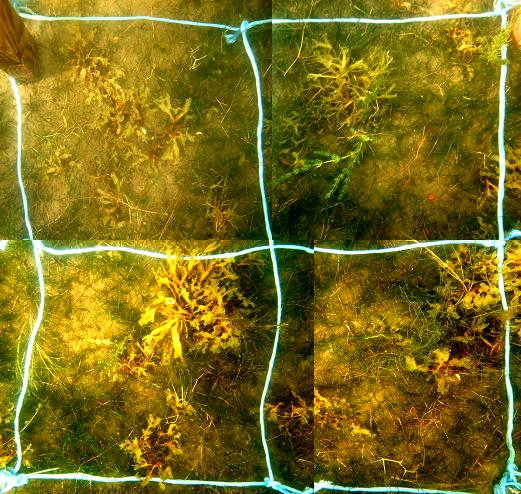
\includegraphics[height=0.55\textheight]{images/Fotos/griebenvonoben.jpg}
\end{figure}
\onslide<2>
\begin{figure}
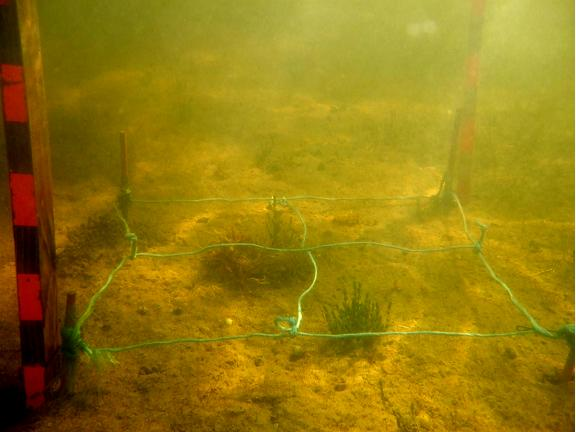
\includegraphics[width=\textwidth]{images/plotpictures/Bsp_G-M}
\end{figure}
\end{overprint}
\end{column}
\end{columns}
\end{frame}


\begin{frame}
\frametitle{PVI}
\begin{columns}
\begin{column}{7.0cm}
\begin{figure}
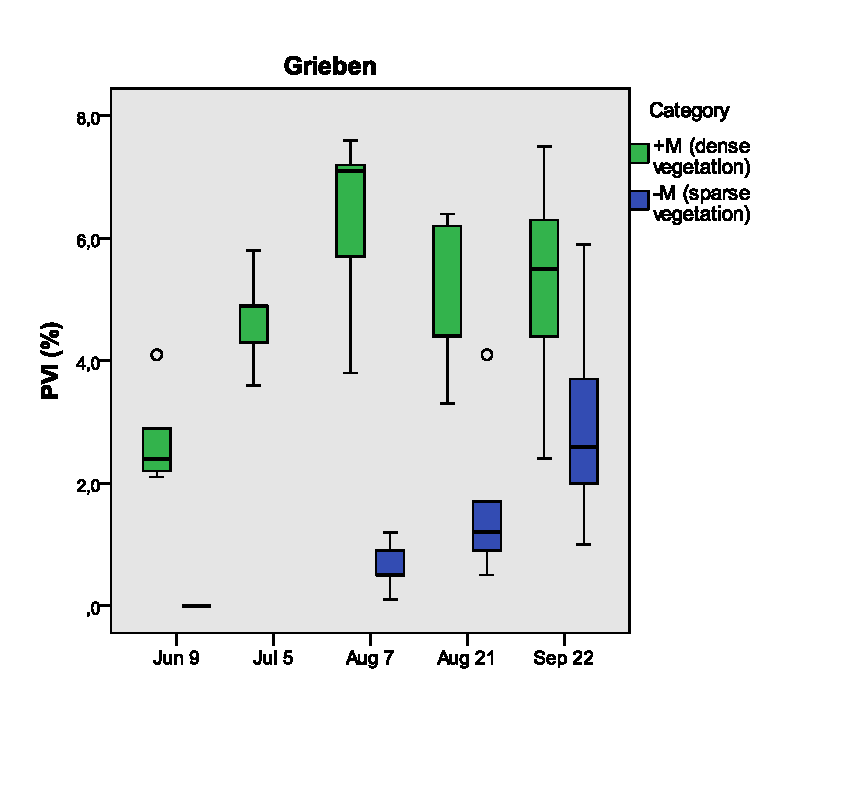
\includegraphics[width=\textwidth]{images/pvi/boxplot_pvi2.eps}
\hspace*{-9mm}
\end{figure}
\end{column}
\begin{column}{5.8cm}
\begin{figure}
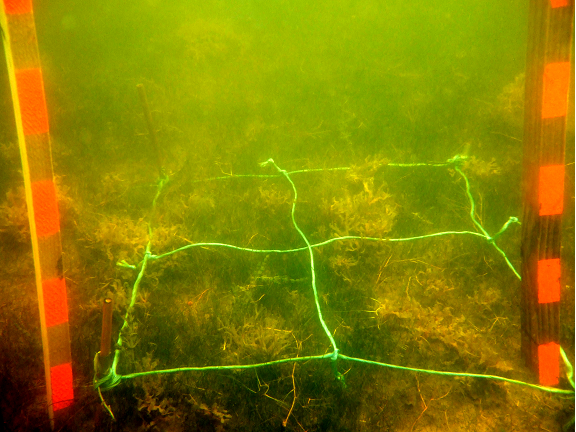
\includegraphics[width=0.9\textwidth]{images/plotpictures/Bsp_G+M}
\hspace*{+9mm}
\end{figure}
\end{column}
\end{columns}
\end{frame}


\subsection{Sediment}

\begin{frame}
\frametitle{Korngrößenverteilungen in Vitte}
\begin{columns}
\begin{column}{5.5cm}
+M
\begin{figure}
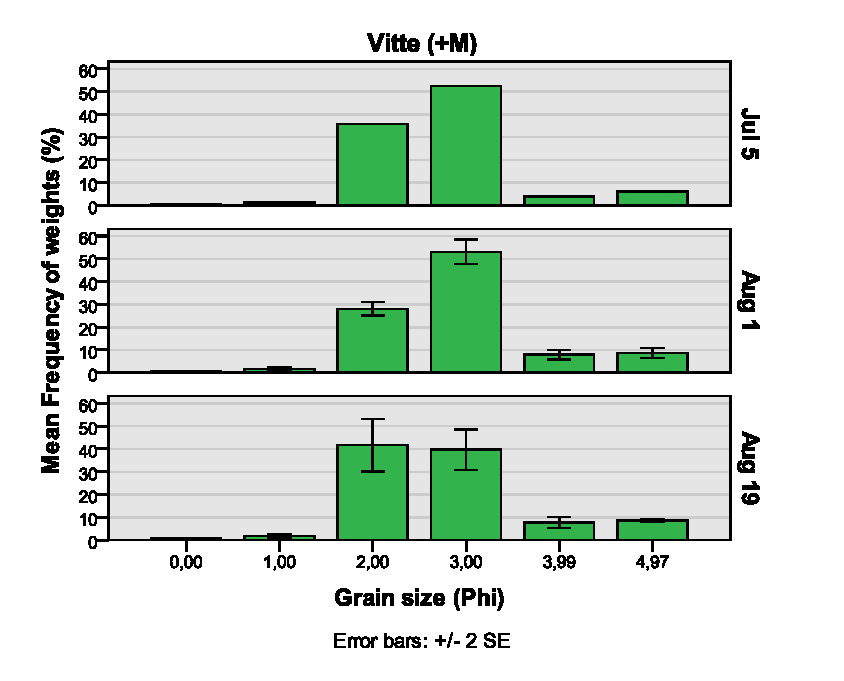
\includegraphics[width=\textwidth]{images/grainsize/sediment_im_jahr1.eps}
\end{figure}
\end{column}
\begin{column}{5.5cm}
-M
\begin{figure}
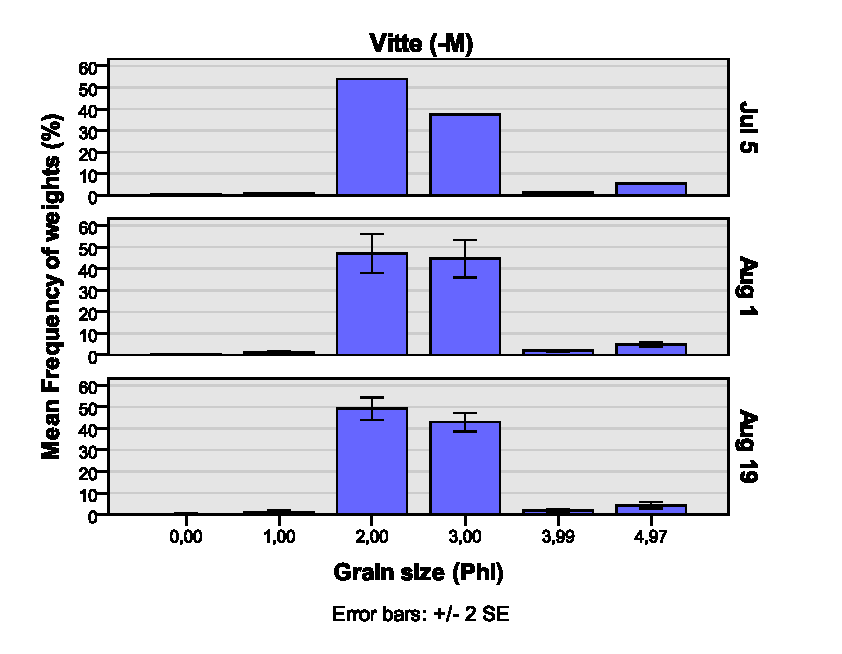
\includegraphics[width=\textwidth]{images/grainsize/sediment_im_jahr2.eps}
\end{figure}
\end{column}
\end{columns}
\end{frame}


\begin{frame}
\frametitle{Korngrößenverteilungen in Grieben}
\begin{columns}
\begin{column}{5.5cm}
+M
\begin{figure}
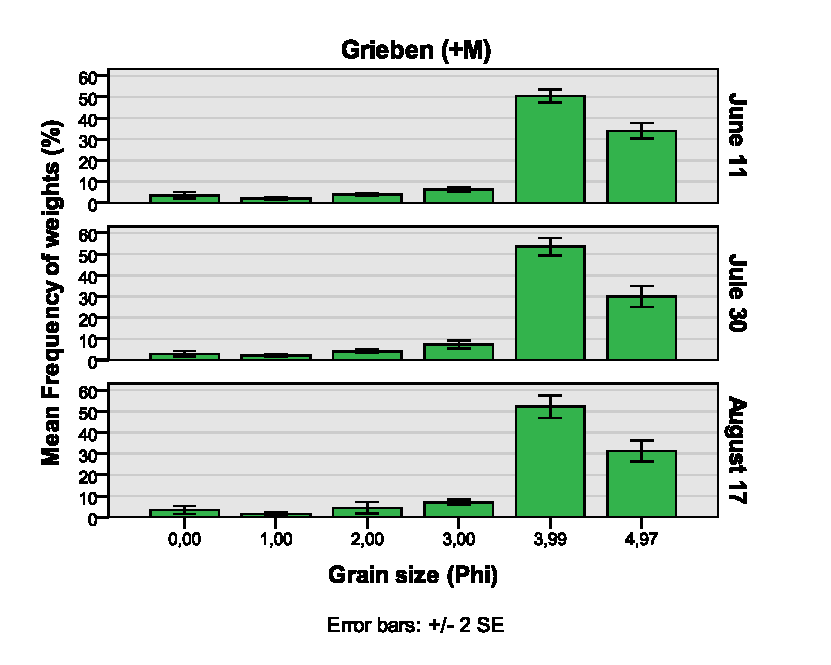
\includegraphics[width=\textwidth]{images/grainsize/sediment_im_jahr3.eps}
\end{figure}
\end{column}
\begin{column}{5.5cm}
-M
\begin{figure}
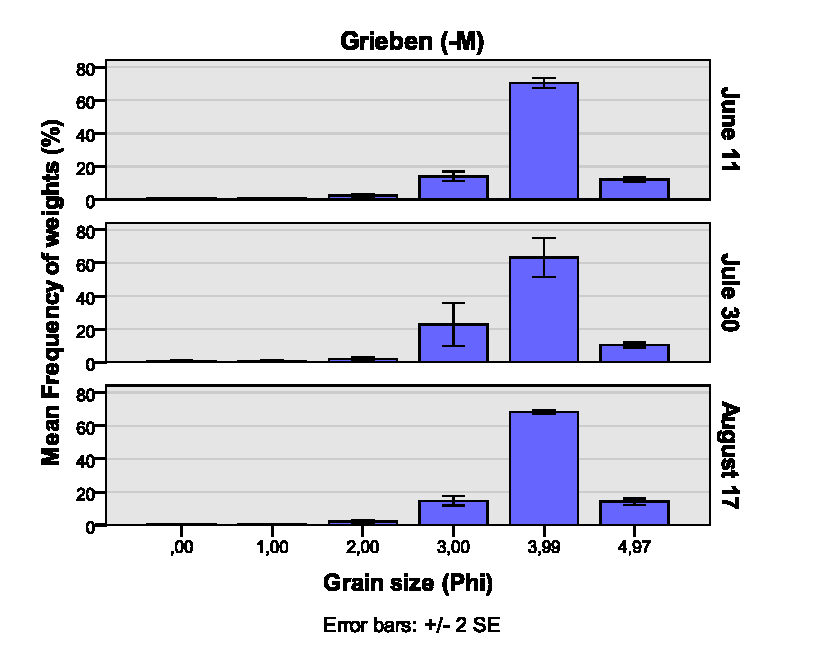
\includegraphics[width=\textwidth]{images/grainsize/sediment_im_jahr4.eps}
\end{figure}
\end{column}
\end{columns}
\end{frame}


\begin{frame}
\begin{columns}
\begin{column}{5.5cm}
Feinpartikulärer Anteil
\begin{figure}
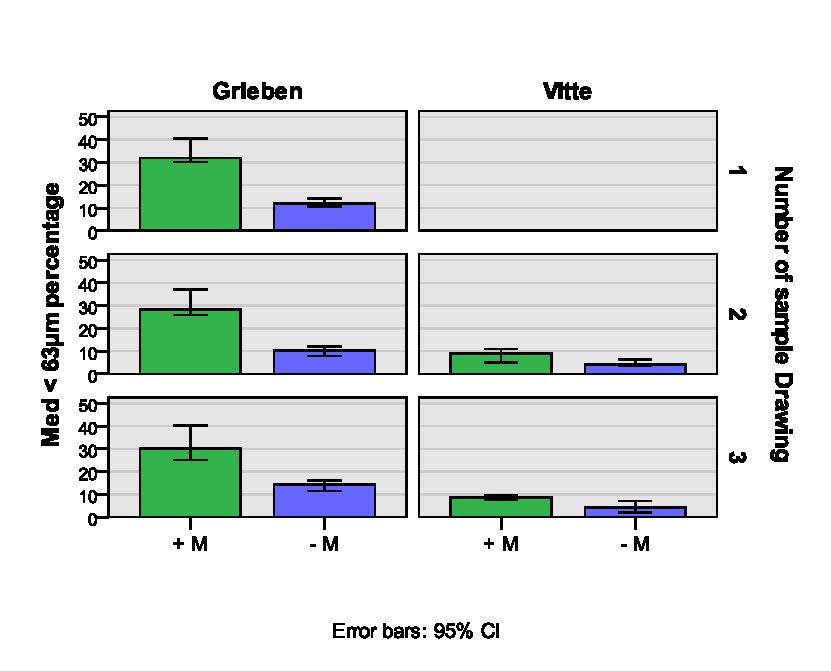
\includegraphics[width=\textwidth]{images/sedimentparameter/S_Parameter_63_neu1.eps}
\end{figure}
\end{column}
\begin{column}{5.5cm}
\pause
Organischer Gehalt
\visible<2>{
\begin{figure}
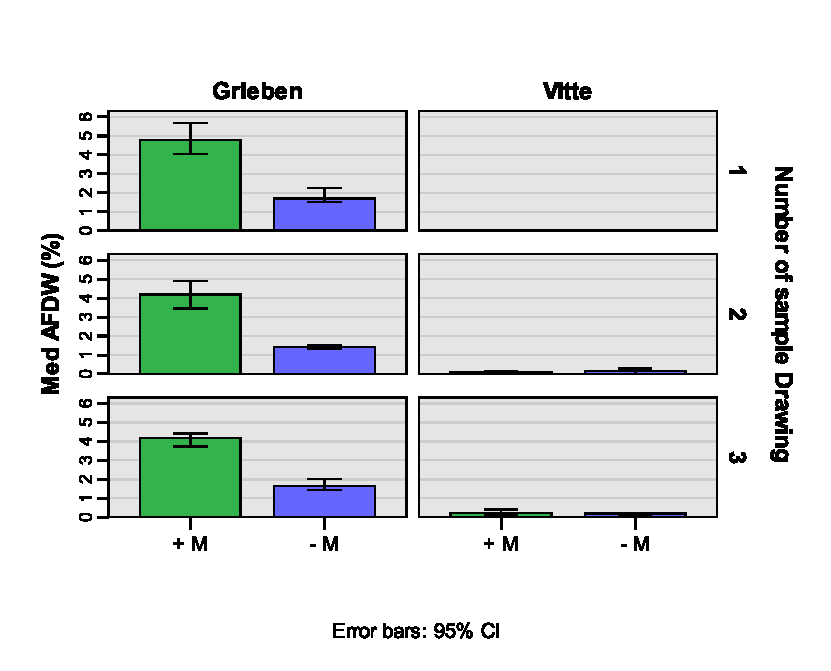
\includegraphics[width=\textwidth]{images/sedimentparameter/afdg_neu1.eps}
\end{figure}}
\end{column}
\end{columns}
\end{frame}

\subsection{Fazit}
\begin{frame}
\begin{columns}
\begin{column}{9.5cm}
\begin{enumerate}[<+->] 
\item Ist in dichten Makrophytenbeständen das Sediment feiner als auf freien/ spärlich besiedelten Flächen?
\item Ist der organische Gehalt der Sedimente in den dichten Beständen höher?
\item Verändert sich die Vegetationsstruktur im Jahresverlauf?
\item Verändert sich die mittlere Korngröße, der Feinpartikelanteil und der organische Gehalt der Sedimente im Jahresverlauf?
\end{enumerate}
\end{column}
\begin{column}{2.5cm}
\begin{itemize}
\item<1->[\cmark] 
\item<1->[] 
\item<2->[\cmark]
\item<2->[]
\item<3->[\cmark] 
\item<3->[]
\item<4->[\xmark]
\item<4->[]
\end{itemize}
\end{column}
\end{columns}
\end{frame}

%\section{Quellen}
%\begin{frame}
%\frametitle{Bildquellen}
%\begin{itemize}
%\item[1] \textsc{Engelen, Bert}, http://%www.pmbio.icbm.de/expeditions/leg301/subproben.jpg 
%[Aufruf 8.5.2014; 13:59]
%\item[2] \textsc{Melbourne Geofabrics}, http://www.treemax.com.au/content/sieves 

%[Aufruf 8.5.2014; 12:18]
%\item[3]  \textsc{Stäuber, Kurt}, 

%http://wisplants.uwsp.edu/scripts/bigphoto.asp 

%[Aufruf 8.5.2014; 14:20]

%\end{itemize}

%\end{frame}


\end{document}

\begin{document}
\begin{frame}
\frametitle{Detaillierte Vegetationsstruktur (dichte Vegetation)}
\begin{columns}
\begin{column}{4.8cm}
\begin{figure}
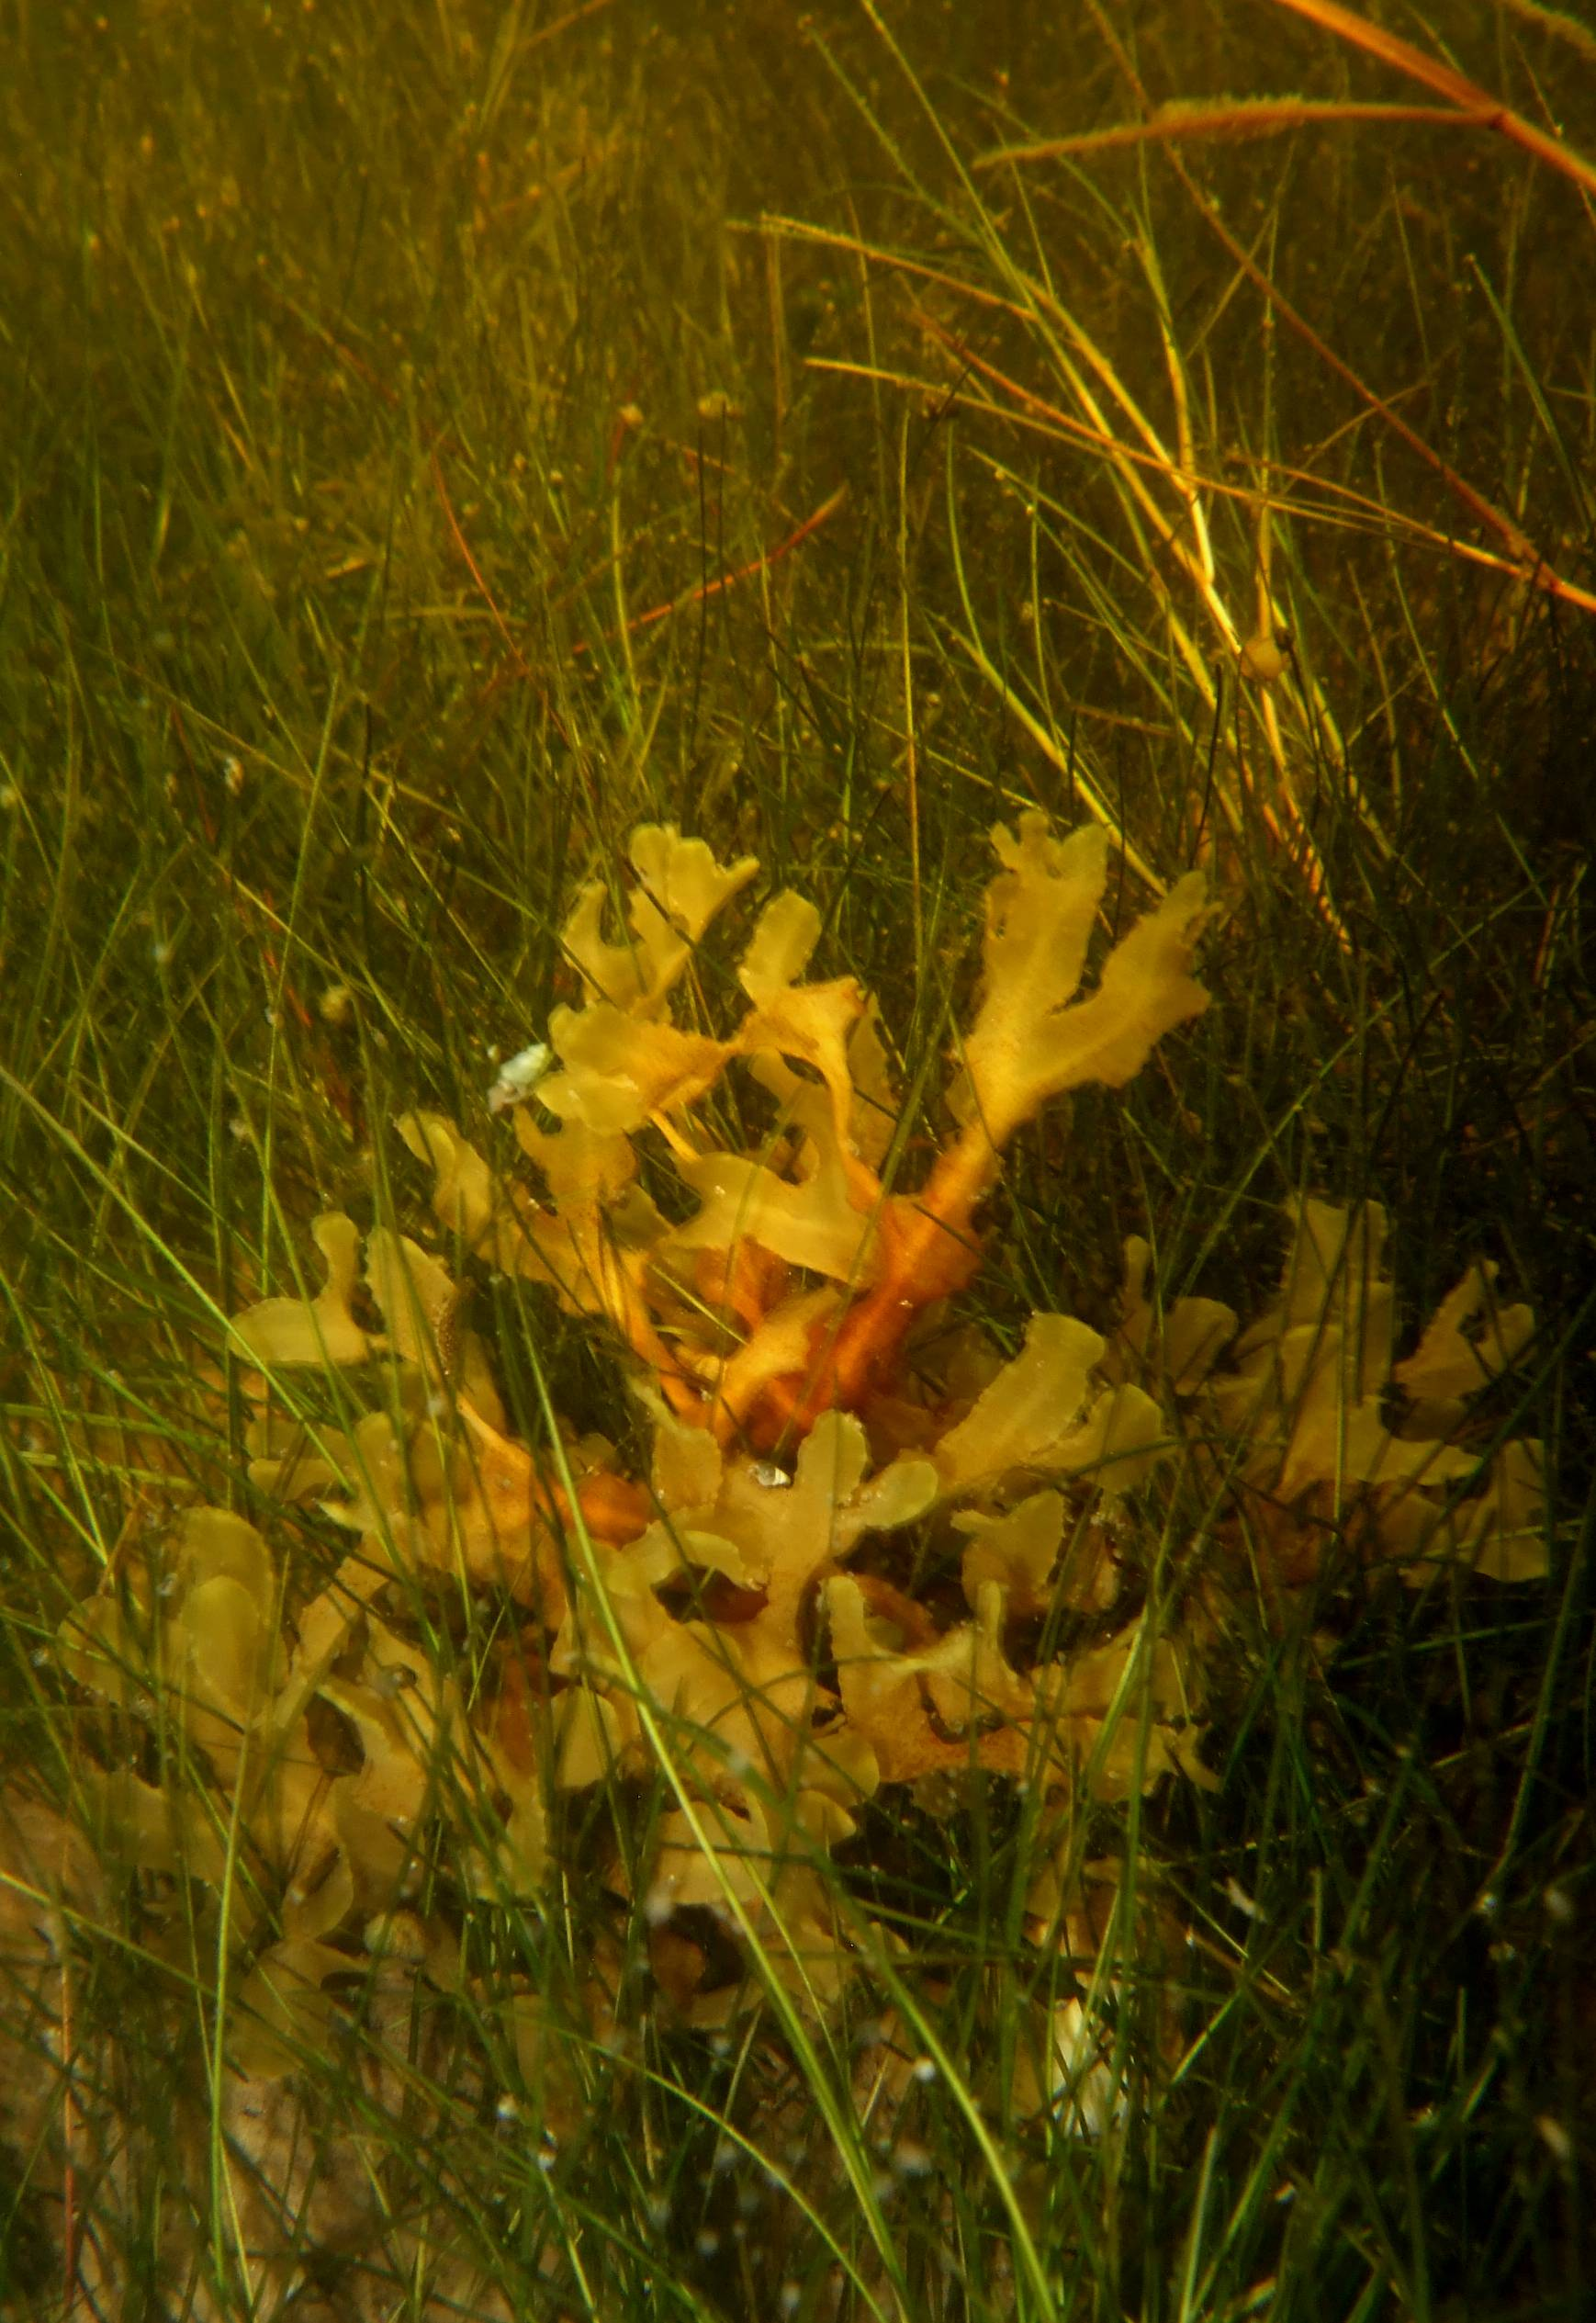
\includegraphics[width=0.7\textwidth]{images/Fotos/DSCF0799.JPG} 
\end{figure}
\begin{center}
Blasentang

(\textit{Fucus vesiculosus})
\end{center}
\end{column}
\begin{column}{8.0cm}
\begin{figure}
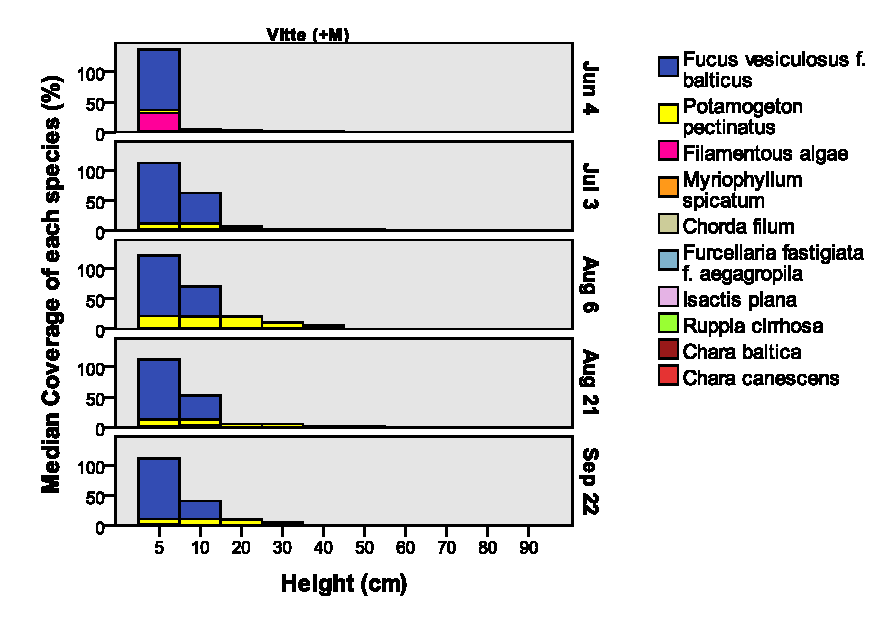
\includegraphics[width=\textwidth]{images/Wuchshoehenkartierung/Vitte+Mb1.eps}
\end{figure}
\end{column}
\end{columns}
\end{frame}

\begin{frame}
\frametitle{Detaillierte Vegetationsstruktur (spärliche Vegetation)}
\begin{columns}
\begin{column}{4.8cm}
\begin{figure}
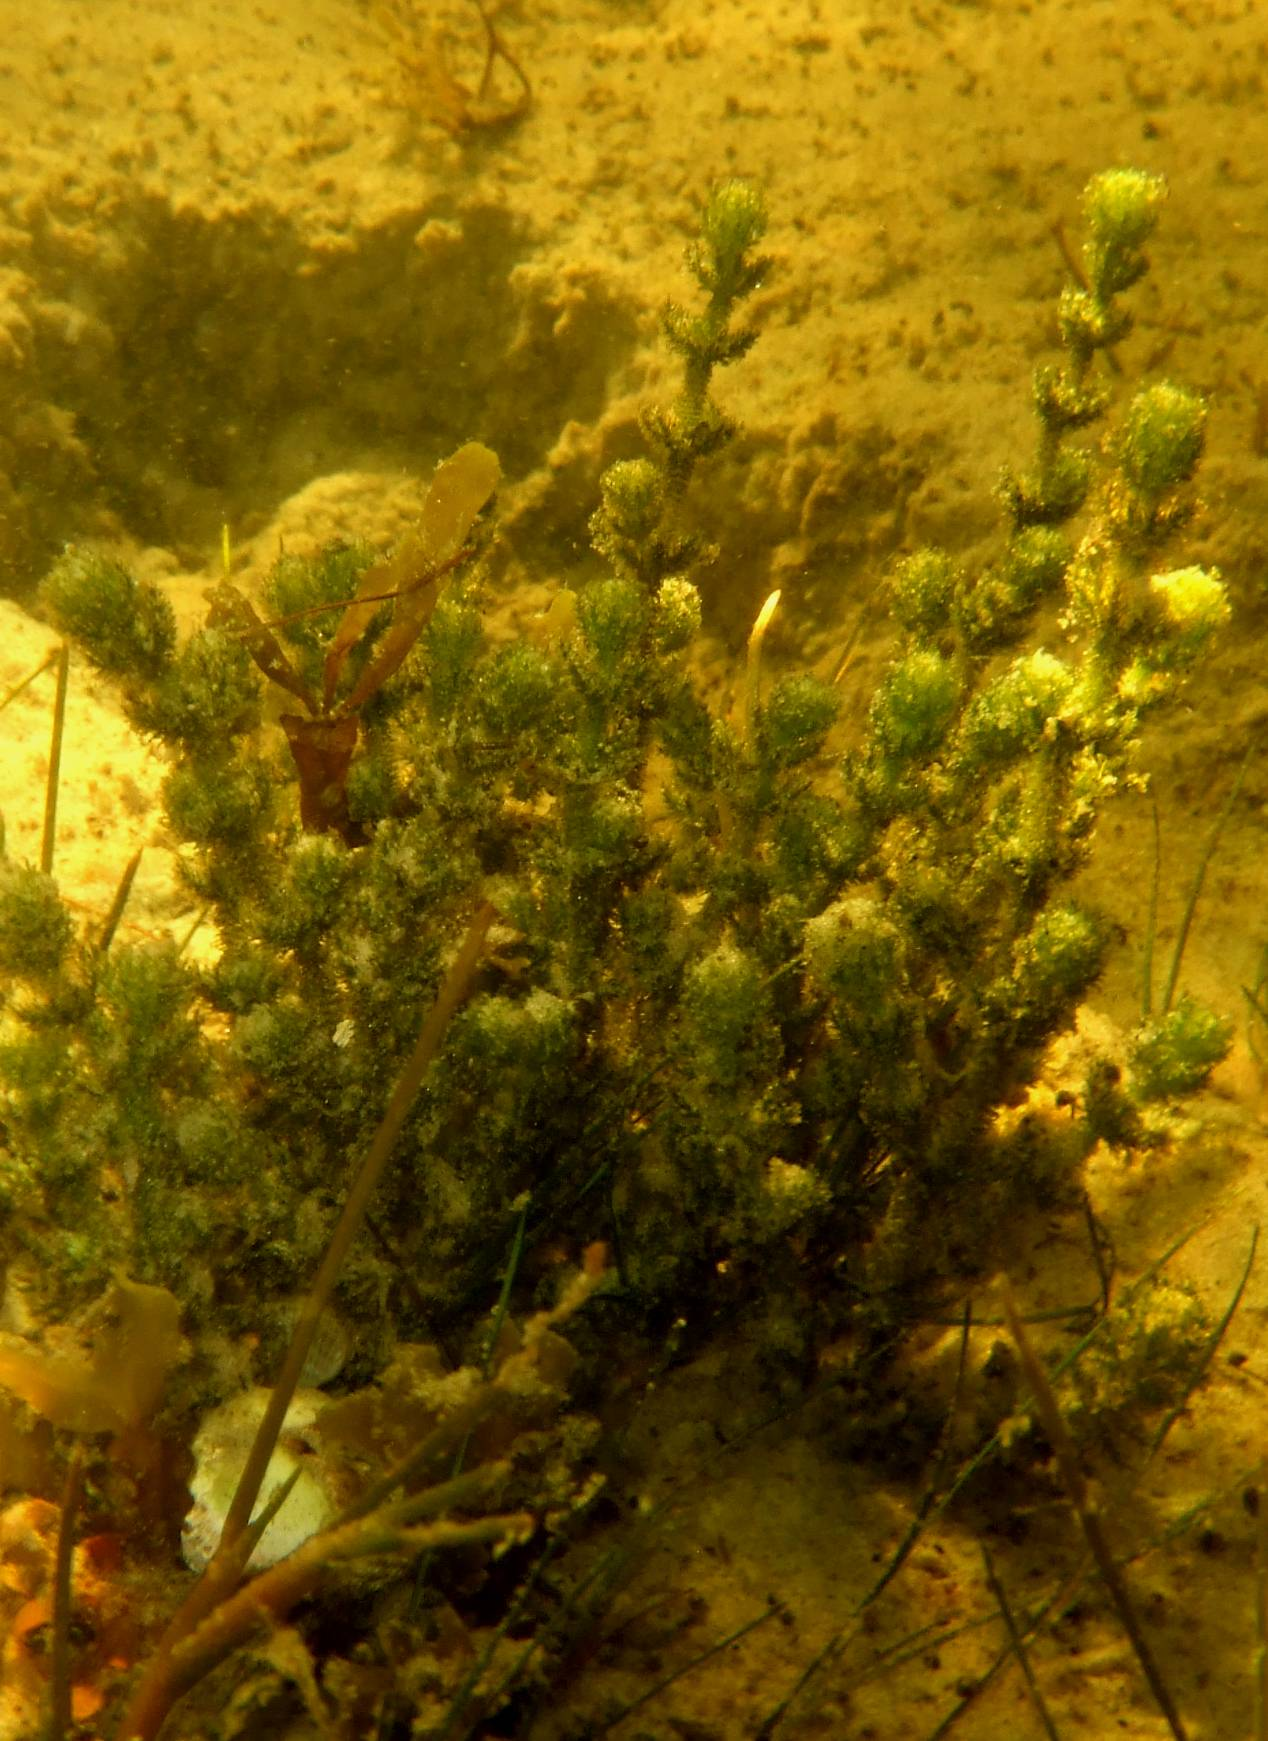
\includegraphics[width=0.7\textwidth]{images/Fotos/DSCF0876.JPG}
\end{figure}
\begin{center}
Armleuchteralge

(\textit{Chara canescens})
\end{center}
\end{column}
\begin{column}{8.0cm}
\begin{figure}
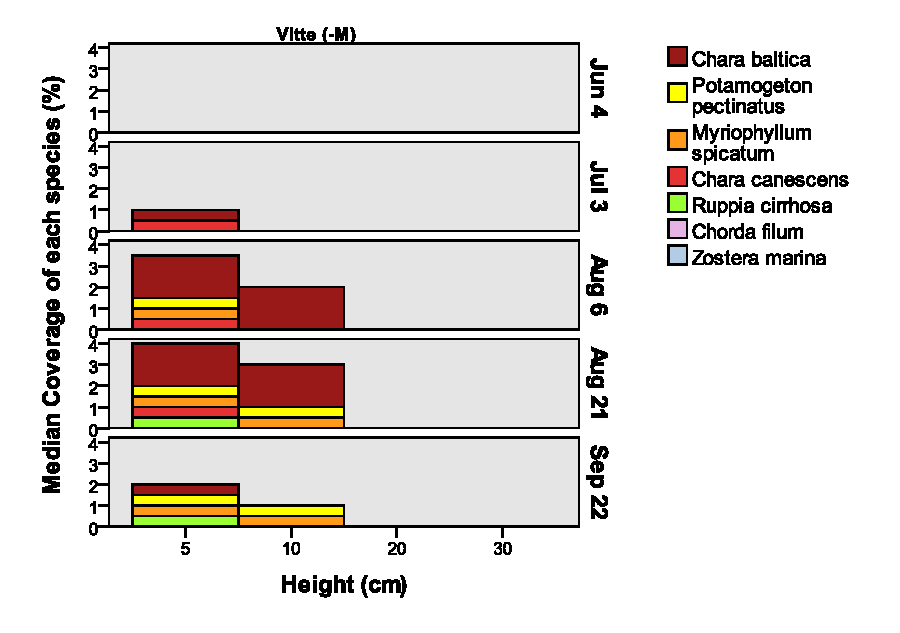
\includegraphics[width=\textwidth]{images/Wuchshoehenkartierung/Vitte-M1.eps}
\end{figure}
\end{column}
\end{columns}
\end{frame}

\begin{frame}
\frametitle{Detaillierte Vegetationsstruktur}
\begin{columns}
\begin{column}{4.8cm}
\begin{figure}
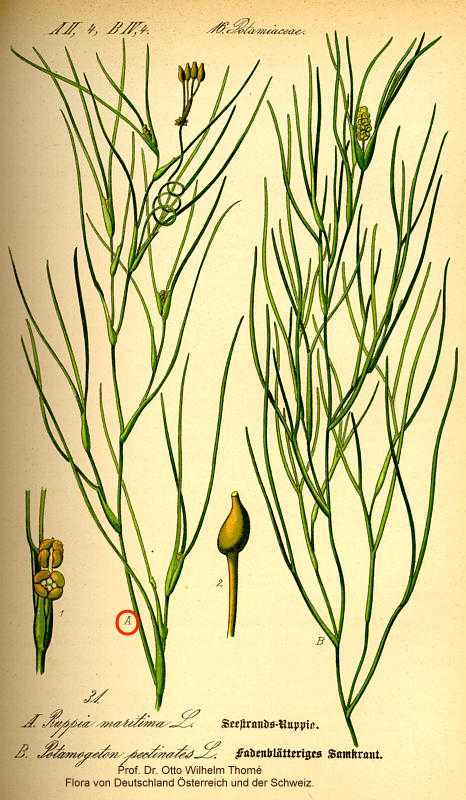
\includegraphics[width=0.6\textwidth]{images/Fotos/ruppia.jpg} {\small [3]}
\end{figure}
\begin{center}
Schraubige Salde

(\textit{Ruppia cirrhosa})
\end{center}
\end{column}
\begin{column}{8.0cm}
\begin{figure}
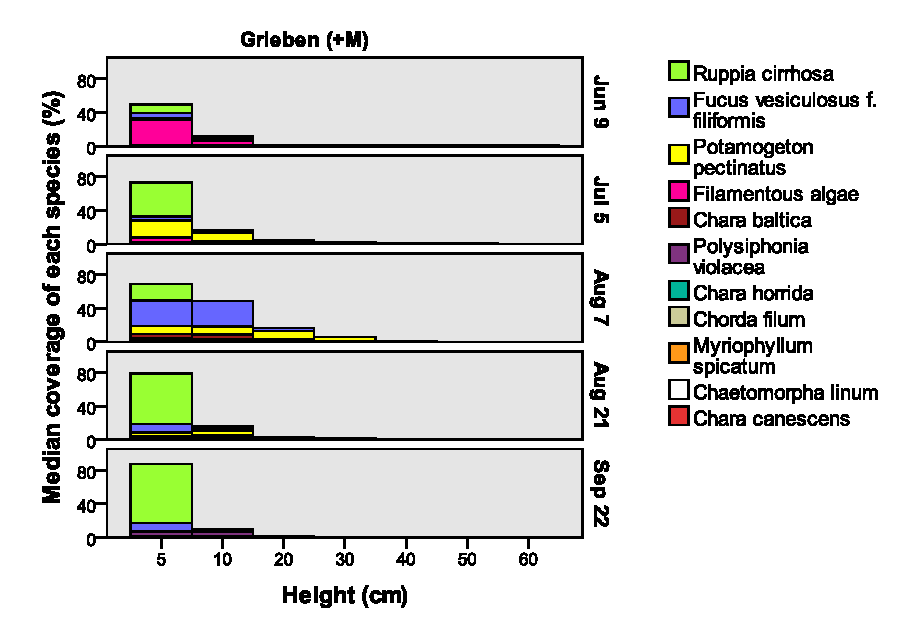
\includegraphics[width=\textwidth]{images/Wuchshoehenkartierung/Grieben+M1.eps}
\end{figure}
\end{column}
\end{columns}
\end{frame}

%\begin{frame}
%\frametitle{Spärlich bewachsene Standorte}
%\begin{columns}
%\begin{column}{5.5cm}
%\begin{figure}
%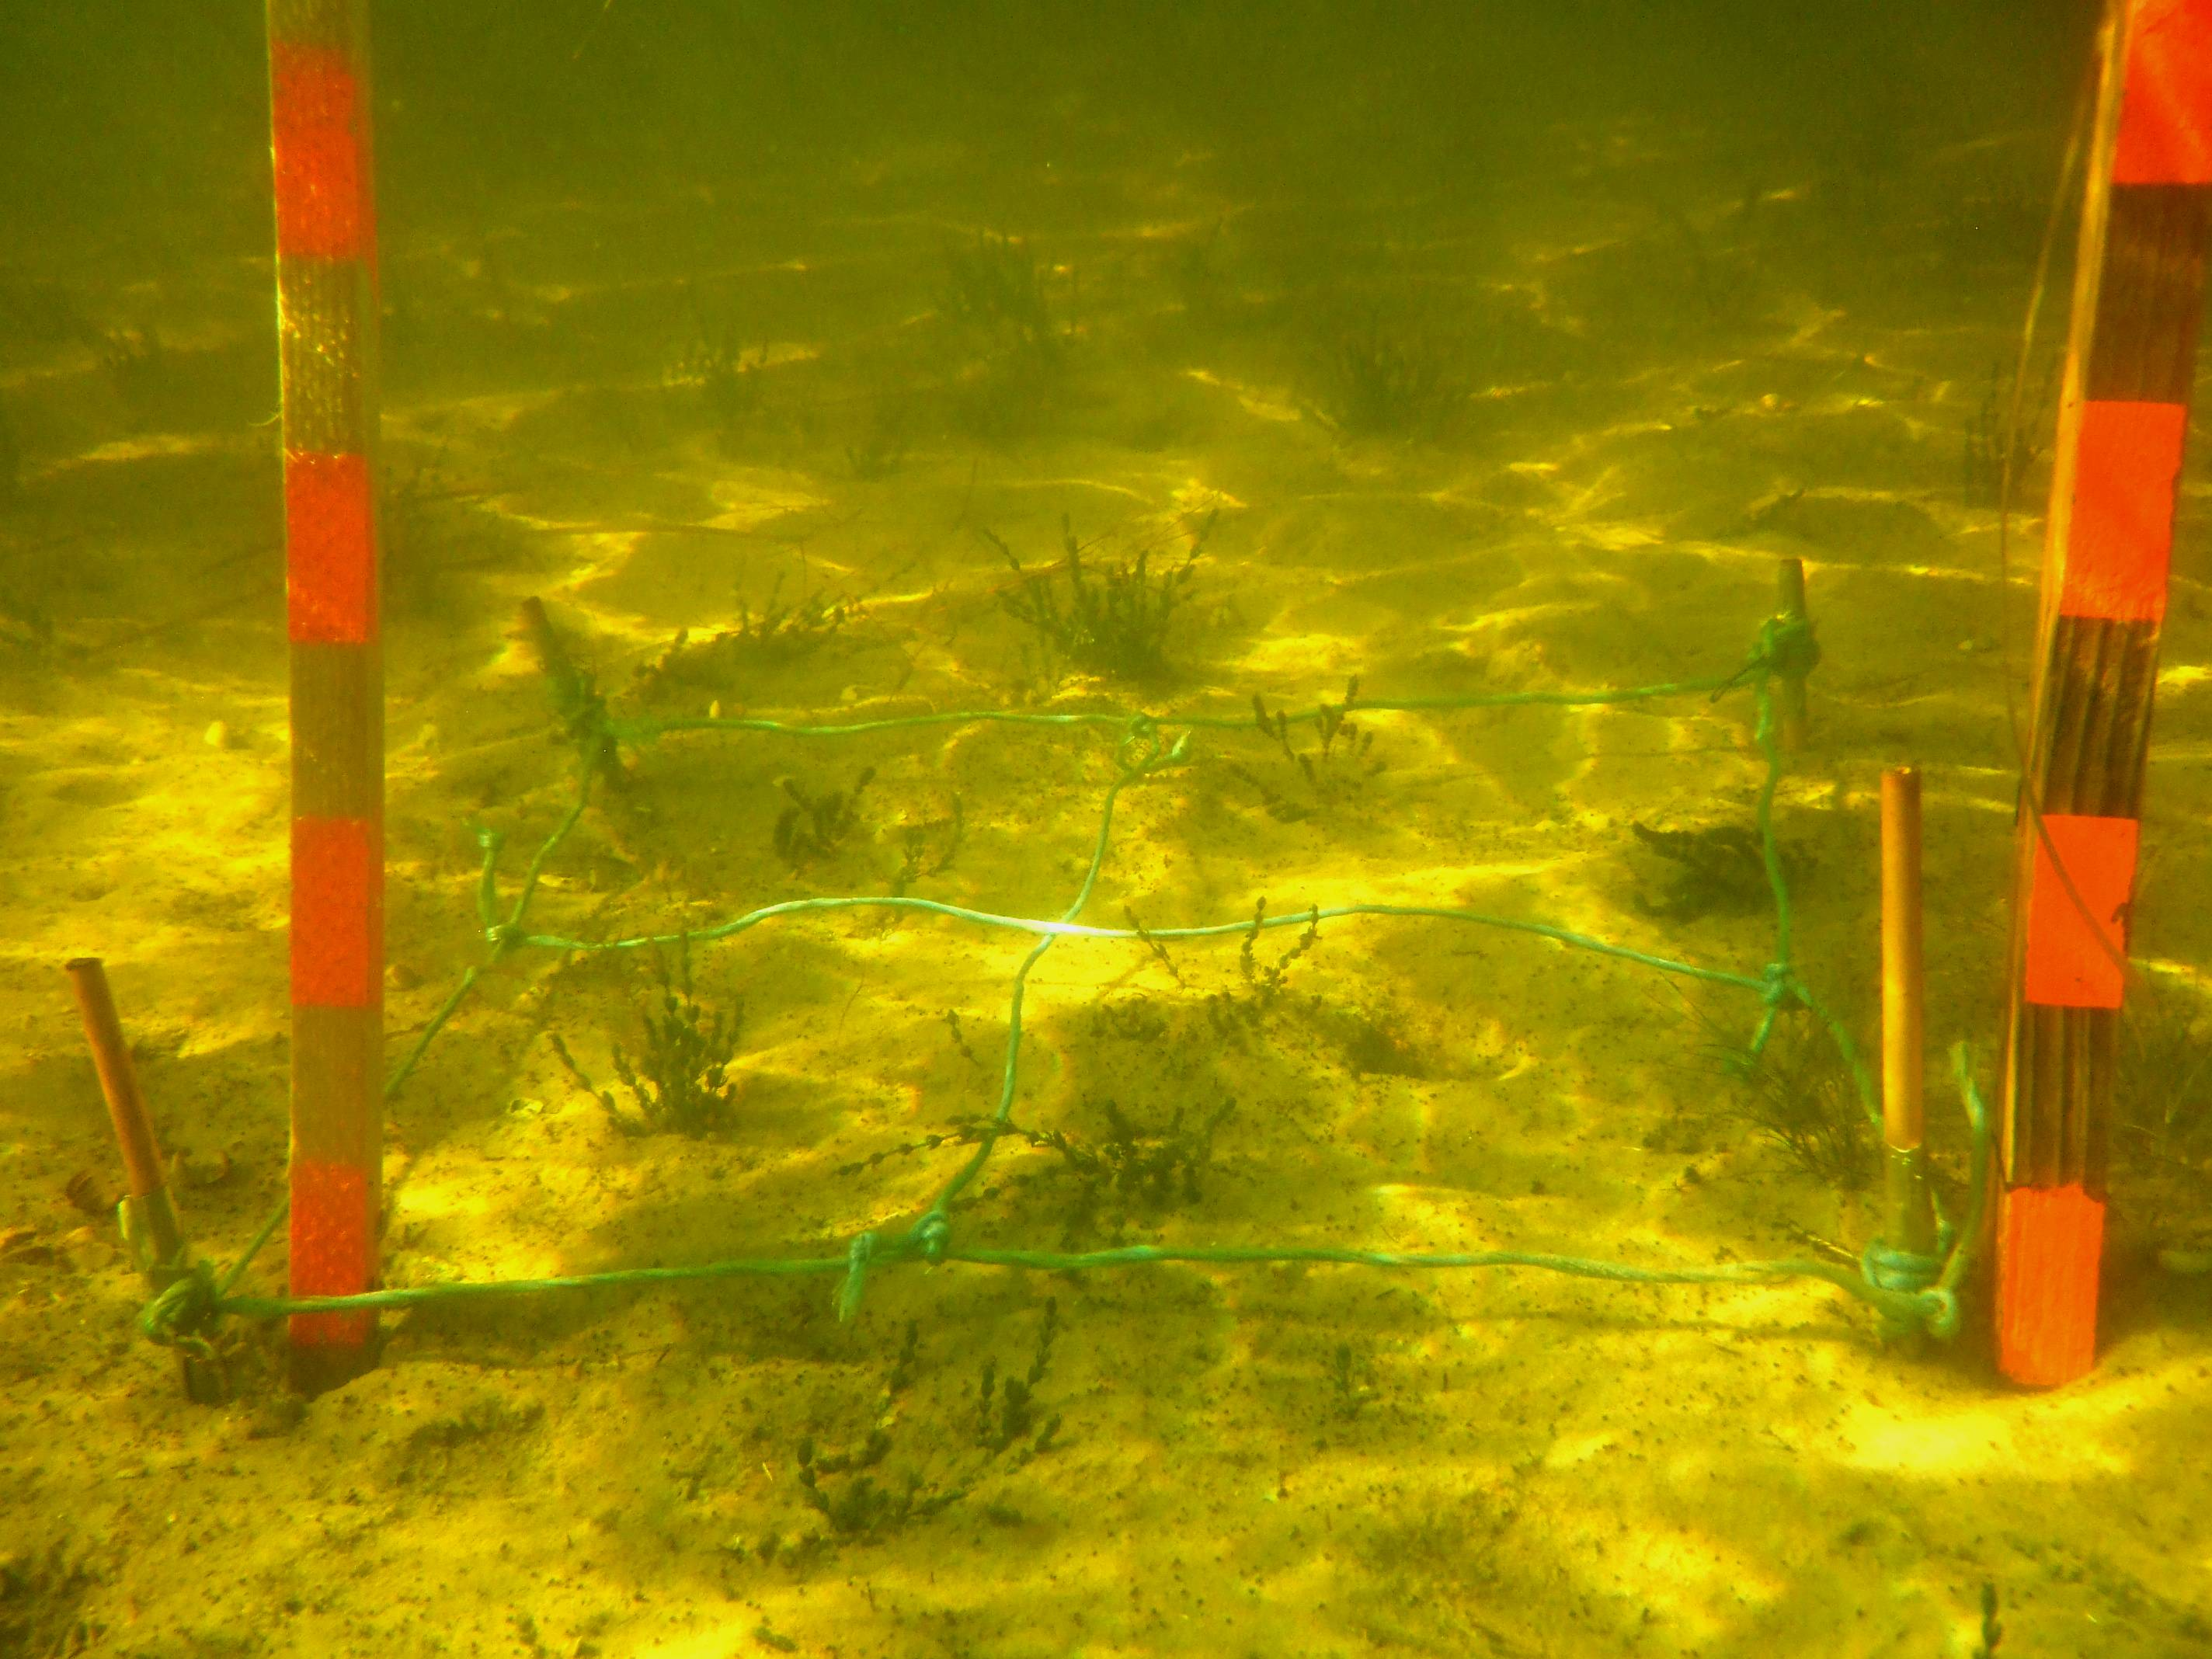
\includegraphics[width=\textwidth]{images/plotpictures/Bsp_V-M}
%\end{figure}
%\end{column}
%\begin{column}{5.5cm}
%\begin{figure}
%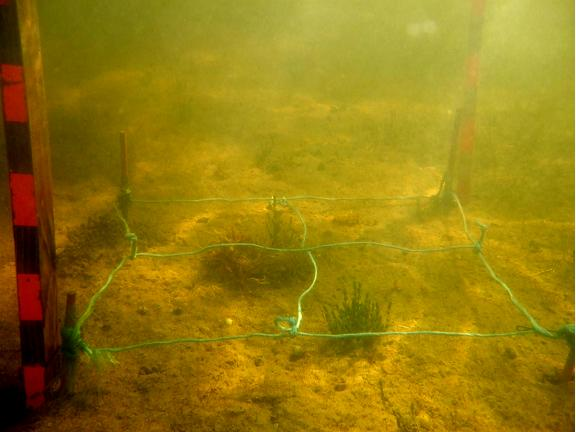
\includegraphics[width=\textwidth]{images/plotpictures/Bsp_G-M}
%\end{figure}
%\end{column}
%\end{columns}
%\end{frame}


\begin{frame}
\frametitle{Grieben (-M)}
\begin{columns}
\begin{column}{4.8cm}

\end{column}
\begin{column}{8.0cm}
\begin{figure}
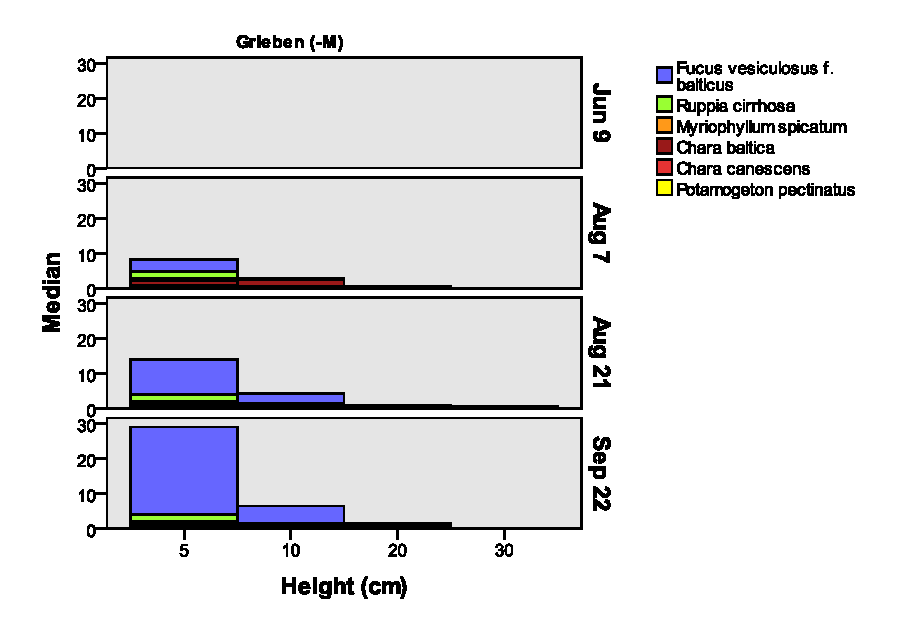
\includegraphics[width=\textwidth]{images/Wuchshoehenkartierung/Grieben-M1.eps}
\end{figure}
\end{column}
\end{columns}
\end{frame}


\end{document}
